\title{Connecting green space supply and demand: modeling the walkable environment of European cities}
\author{Benjamin Labohm}
\documentclass[10pt]{article}
\usepackage{geometry}
\geometry{a4paper, top=25mm, left=20mm, right=20mm, bottom=25mm,
headsep=10mm, footskip=12mm}
\setlength{\parindent}{0em} 
\usepackage{setspace}
\onehalfspacing
\usepackage{url}
\usepackage{hyperref}
%\usepackage{microtype}
\usepackage{natbib}
%\usepackage{subcaption}
\usepackage[english]{babel}
%\usepackage{multirow}
\usepackage{booktabs}
\usepackage{graphicx}
\usepackage{float}
%\usepackage{lscape}
%\usepackage[toc,page]{appendix}
\graphicspath{{D:/MA/plots/}}

\begin{document}
\emergencystretch 3em
\onecolumn

{\center
\vspace*{5cm}
{\Huge Connecting green space supply and demand: modeling the walkable environment of European cities}
\par\bigskip
\Large{
\textbf{Master's thesis}\\
Humbold-Universit\"at zu Berlin

Geography Department
\\
Benjamin Labohm

Mat. Nr.: 
545609
\vfill
}
}
\large{


Supervisors: \\
Prof. Dr. Dagmar Haase

Humbold-Universit\"at zu Berlin

Geography Department\\


Dr. Manuel Wolff

Humbold-Universit\"at zu Berlin

Geography Department \\

Berlin, 15.07.2022
}

\newpage
\normalsize
\tableofcontents
\newpage
\listoffigures
\newpage

\twocolumn[{\centering{\huge Connecting green space supply and demand: modeling the walkable environment of European cities\par}\vspace{3ex}
	{\large Benjamin Labohm*\par}\vspace{2ex}
	\today\par\vspace{4ex}}
\textit{\small{*Geography Department, Humbold-Universit\"at zu Berlin, Rudower Chaussee 16, 12489 Berlin}} \\
\smallbreak
\hrule 

\vspace*{.5cm}

\textbf{Abstract}

In an increasingly urbanized world, peoples’ access to urban green spaces (UGS) is crucial. 
Former studies have mostly focused on determining whether urban dwellers have access to UGS or not.
We used network characteristics to analyze the walkable environment – the connecting area between green space demand and supply – of European cities. 
By employing the Local Significance (LS) index, we revealed potential overcrowding effects at UGS in southern Germany.
With the Detour Index (DI), we could not only show how many urban residents have access to UGS within 500 meters network distance, but also estimate the efficiency of the routes people take. 
To make the workflow replicable for future analysis, we used open source data and software.
Future research should focus on i.) accounting for the number of UGS people can reach, ii.) augment our results with further environmental data and iii.) account for other means of transportation, like cycling or public transport.

\vspace*{.5cm}

\hrule

\par\vspace{2ex}]

\vspace{.5cm}

\normalsize


\section{Introduction}
%Part1: Accessibility to UGS
In the Anthropocene, rapid urbanization takes place globally. 55\% of the global population were living in cities by 2018 and 68\% are projected to do so in 2050.
A growing urban population depends increasingly on urban ecosystems \citep{Elmqvist.2021, UN.2019}.
Ecosystems supply ecosystem services (ES) which are critical to human well-being \citep{Fisher.2009}.
Living in proximity of urban green spaces (UGS) can help alleviate the impacts of climate change on and aging urban population, as well as improve overall public health in cities \citep{Kabisch.2021, Kabisch.2021b}.
Thus, having access to UGS can enhance urban inhabitants’ quality of life \citep{Poelman.2018}.
Likewise, the United Nations have agreed to provide universal access to public green spaces by 2030 in Sustainable Development Goal 11.7 \citep{UN.2017}.

In Europe, 74\% of the population are living in cities \citep{UN.2019}.
Here, the population pressure on UGS might be amplified by the compact city paradigm, which is popular among European city planners: A more compact city can result in shorter traveling distances but also in more overcrowding effects (Commission of European Communities, 1990; Burton.2003, Wolff.2019).
Accordingly, more people living in proximity to and benefitting from an UGS also increase the pressure on its ecological functions \citep{Wolff.2019}.
In order to detect such mismatches in green space supply and demand and to provide equal access to UGS, mapping UGS accessibility is key \citep{Larondelle.2013}.

The walkable environment – the space in between urban dwellers and UGS – not only affects the quality of ES and, thus, the accessibility of UGS \citep{Syrbe.2012}.
Availability of UGS in walking distance can improve overall public health and increase the resilience of city dwellers \citep{Kabisch.2021,Richardson.2013}.
A proper modeling of UGS accessibility must, therefore, put emphasis on modeling the walkable environment of a city \citep{Wolff.2019}.
Yet, easy to use and open source tools for comparatively modeling the walkability of European cities are lacking \citep{Kabisch.2016}.

%Part 2: State of the art
Availability and accessibility of UGS in Europe have been analyzed and compared in multiple studies.
In their 2016 paper, Kabisch et al. carried out an assessment of green space availability in 299 EU cities. They used a population grid of 1 km² and land use data (urban atlas) to calculate the population within a buffer distance of UGS \citep{Kabisch.2016}.
The use of Euclidean (direct) distance in accessibility analysis has been found to underestimate spatial distances and to overestimate the provision of UGS in contrast to using network distance, though \citep{Sander.2010, Moseley.2013}.
In 2016, the Joint Research Center (JRC) of the European Union developed an indicator for areas that are served by UGS in European cities. In their analysis, the authors used a 10 m² resolution land use data grid and a 100 m² population mosaic and a network-based approach \citep{Pafi.2016}.
In another analysis from 2018, the JRC used urban atlas data and a street network to assess the area that urban dwellers can reach in a walking distance of 10 minutes. Their analysis also resulted in an area per population measure on a city level \citep{Poelman.2018}.
Wolff and Haase looked into the connection between green space supply and residential density in 905 European cities. They found a strong link between residential density, population size and location of the cities \citep{Wolff.2019}.
Further studies have developed methods to account for problems associated with fixed catchment sizes by using variable catchment approaches \citep{Luo.2012}.

In a 2021 paper, Wolff coupled the population pressure and proximity perspectives by applying network characteristics. In his analysis, he found two promising indicators, the Detour Index (DI) and the Local Significance (LS) \citep{Wolff.2021}.
The DI is a measure of the efficiency of a route taken to reach a goal \citep{Barthelemy.2018}.
Hence, the DI can be used to model barriers that people have to overcome on their way to UGS \citep{Wolff.2021}.
The LS is a simple measure to describe the relevance of different edges of a network \citep{Esch.2014}.
With a little modification, the LS can be utilized to model use-intensity of those edges connecting population demand with UGS. As a consequence, LS might serve as a spatial indicator for overuse of UGS \citep{Wolff.2021}.

Previous research did rarely account for the mutual dependencies of supply and demand, or did it put the focus on the walkable environment \citep{Syrbe.2017}.
Using fixed distances for assessing green space accessibility might lead to numerical quantities instead of focusing on the location of the mismatch between ES supply and demand \citep{Higgs.2012, Syrbe.2017}.
Furthermore, we saw mostly one perspective being used to assess green space accessibility (provision, population pressure or proximity).
But a high provision of UGS in a city, for example, does not necessarily indicate an equal or adequate distribution of UGS \citep{Poelman.2018}.

In addition to the previous points, the mentioned studies, if on a larger scale, were carried out on a coarse resolution (Kabisch et al. 2016, European Commission 2016).
A higher resolution can reveal spatial patterns at a finer scale enabling targeted intervention while also reducing uncertainties that are introduced by e.g. a population grid or a city block aggregation as in urban atlas data \citep{Barthelemy.2018, Esch.2014}.
Achieving a high resolution on a large scale can be challenging, though, since freely available and comparable datasets are scarce \citep{Feltynowski.2018, Dworczyk.2021}.

All things considered, knowledge about green space accessibility is important for planning and decision making and mapping the capacity, flow and demand of ES in urban areas has been found to facilitate urban planning \citep{Baro.2016}.
Improving the modeling of the walkable environment with a combination of population pressure and proximity aspects of green space accessibility might prove promising to detect mismatches between UGS supply and demand \citep{Biernacka.2019, Biernacka.2020}.
Finally, municipalities across European countries still provide a mixture of different indices for measuring green space supply and demand (Kabisch et al. 2016).
Comparing cities can provide a basis for better understanding of urban processes, though \citep{Wolff.2020}.
Yet, there is no easy-to-handle and comparable tool using a high resolution on a European scale with publicly available data and software.


\section{Conceptualization}
The availability of UGS can be defined by the “amount of green area in a defined distance to where urban residents live” \citep{Kabisch.2016}.
Having actual access to UGS might be limited by additional factors, though. 
The physical accessibility, for example, can be limited by fences, opening hours of an UGS, or the detours people have to take to reach them. 
Additionally, accessibility may be limited by perceived overcrowding effects through population pressure \citep{Kabisch.2016, Wolff.2020b}.
As use intensity can influence ES, it can create a mismatch between supply and demand \citep{Syrbe.2017}. 

Approaches that accounted for the supply and demand aspects of ES have usually postulated a population that is close to the places of ES origin. 
Since ES are rarely consumed by humans at the same place where they are produced by the ecosystem, we distinguish service providing areas (SPA) and service demanding areas (SDA). 
Service providing areas (SPA) represent the supplying side, the spatial unit where the ES are generated \citep{Syrbe.2012, Dworczyk.2021}.
In cities, UGS supply for example the cultural ES of recreation for residents \citep{Dickinson.2017}.
Service demanding areas (SDA) embody the places where the potential demand for ES arises, e.g. the places where people live. In the case of UGS in an urban environment, residential areas or buildings are an example for SDA \citep{Dworczyk.2021}.

In order to account for physical and perceived barriers to green space access, we have to take a look at the space between SPA and SDA, the service connecting areas (SCA).
SCA can be used to show the flow of ES between SPA and SDA areas \citep{Syrbe.2012, Dworczyk.2021}.
Regarding the scenario of UGS in cities, SCA are the walkable environment, i.e. the routes residents take to benefit from the ES in their neighborhood \citep{Syrbe.2017}.
Consequently, the SCA in this case are the walkable street network of a city.

Three perspectives have been used in past studies to model the SCA for UGS: The proximity, provision and pressure perspectives.
The proximity perspective considers the space between supply and demand, e.g. the walking distance between people’s homes and the UGS, thus highlighting the SCA. 
A proximity perspective is necessary to account for barriers and other characteristics of the network. \citep{Higgs.2012, Wolff.2021}.
Furthermore, green space proximity measures have been found to be among the most important factors influencing perceived accessibility, especially for minority groups \citep{Ibes.2015, Wang.2015}. 
The widely used green space provision perspective models the flow from green area to buildings, thus, focusing on UGS provision (area / person).
Secondly, the less often used population pressure perspective describes the flow from residential buildings (i.e. the population) to the UGS.
The focus here is on the pressure of the residents on an UGS or their demand for green areas (person / area) \citep{Kimpton.2017}.

%Part 3: Objectives
Modeling the walkable environment of European cities by including the three perspectives mentioned above and using a network characteristics approach.
We want to answer the questions:

    1.) What does a modeling approach look like that estimates the walkability between green space supply and demand in cities based on high resolution data? 
    
    2.) How to incorporate publicly accessible data and open source software in order to allow i.) a reproduction over time (e.g. with more recent data), and ii.) comparative approaches covering a large sample of cities.
    
    3.) How can easily understandable and applicable indicators be used in order to support urban planning in detecting mismatches between demand and supply?
    
The objectives that we derived from these questions are i.) to develop a modeling approach that applies walkability indices, ii.) to compare the results on a European scale, and iii.) to implement the indices by showing possible use cases for city planners.



\section{Methods and Data}
\begin{figure*}[t!]
\centering
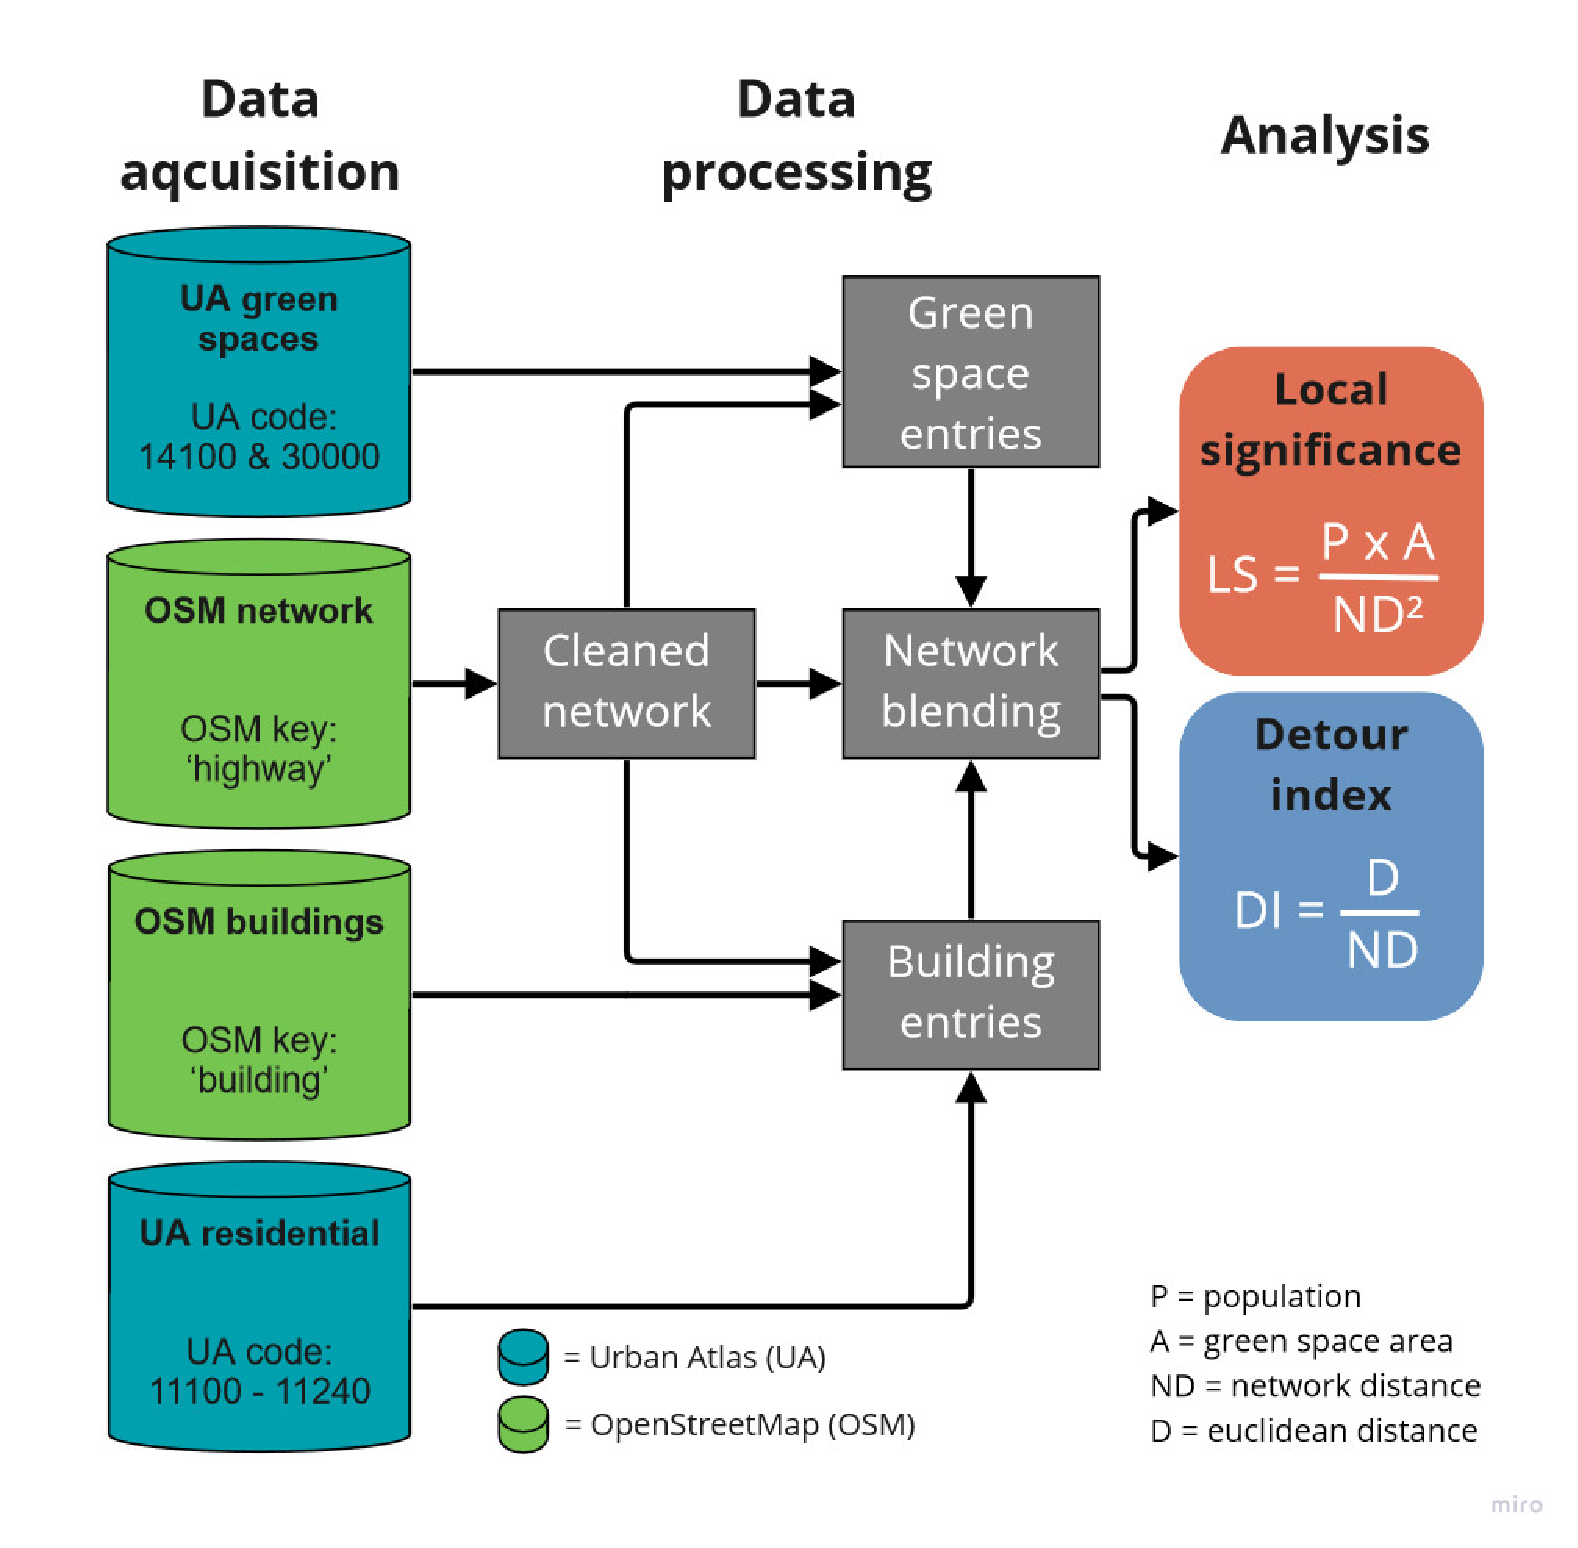
\includegraphics[width=0.6\textwidth]{2-2_md-flowchart.pdf}
\caption{Workflow of data aquisition, processing and analysis (short version). For an exhaustive version of the workflow see appendix 1a.}
\label{fig:flowchart}
\end{figure*}

We applied our analysis to 832 European cities.
To account for the ability of city dwellers to leave their city if they live in proximity to a city border, we included UGS from a buffer of 1 km surrounding the city boundary \citep{Wolff.2020}.
The city delineation stems from the Urban Audit dataset of the European Union \citep{UrbanAudit.2022}.

\begin{table}[h!]
\centering
\resizebox{\columnwidth}{!}{%
\begin{tabular}{@{}lll@{}}
\toprule
source                                                                & data                                                                                        & coverage                                                     \\ \midrule
\begin{tabular}[c]{@{}l@{}}Eurostat\\ Urban Audit\end{tabular}        & city boundaries                                                                             & \begin{tabular}[c]{@{}l@{}}832 cities \\ Europe\end{tabular} \\
OpenStreetMap (OSM)                                                   & \begin{tabular}[c]{@{}l@{}}residential buildings\\ network\end{tabular}                     & global                                                       \\
\begin{tabular}[c]{@{}l@{}}Copernicus\\ Urban Atlas (UA)\end{tabular} & \begin{tabular}[c]{@{}l@{}}urban green spaces\\ residential areas\\ population\end{tabular} & \begin{tabular}[c]{@{}l@{}}788 FUAs\\ Europe\end{tabular}   
\end{tabular}
}
\caption{Overview input data sources and respective data coverage (see appendix 1 for exhaustive version}
\label{tab:data}
\end{table}


\subsection{Data}
For the analysis of the walkable environment of European cities, we needed available and comparable data on public green spaces and residential buildings and their respective entry points.
Additionally, the analysis required information on the population living in each residential building and a network that connects the buildings with the green spaces.
We aimed to incorporate publicly accessible data and open source software in order to allow i.) reproduction (e.g. with more recent data) and ii.) comparative approaches covering a large sample of cities.
We used Urban Atlas (UA) 2018 and OpenStreetMap (OSM) as our main data sources.
All analysis was carried out and tested in R 4.1.3 using RStudio version 1.4.1717 and are made available on the GitHub repository www.github.com/blabohm/MA.
To ensure the best possible data coverage, we downloaded the latest version possible of OSM (April / May 2022).

Urban Atlas (UA): UA is a land use / land cover (LULC) product from the Copernicus program of the European Union.
The 2018 UA version provides Europe-wide comparable data for 788 Functional Urban Areas with more than 50.000 inhabitants.
It represents 17 urban and 10 rural LULC classes with a MMU of 0.25 and 1 ha, respectively.
In addition to the spatial data, UA contains information on the population for the residential land use classes.
Since Copernicus does not offer an API, we downloaded the latest UA version available at the time of this study (c13) by hand.

OpenStreetMap (OSM): OSM is a community-based project that provides free geospatial data.
The OSM community seeks to create a database of the entire planet that is free and editable.
For the analysis we downloaded the OSM data with the identifiers ‘building’ and ‘highway’.
Since OSM is a community-based mapping service, the latest version of OSM data is expected to have the most information.
We acquired the OSM data via the OSM API, which we accessed via a custom-made tool that heavily relies on the R package ‘osmdata’.
For information on the OSM download tool, see Appendix 1c.

\subsection{Data processing}
Street network: The network, in this analysis, represents the walkable environment of a city, which connects the entry points of the UGS with those of the residential buildings.
To acquire information on the street network of a city, we downloaded OSM data with the identifier ‘highway’, which represents all linestrings in the OSM database that are associated with streets and paths.
To secure comparability across European countries, we used all OSM highway classes, except for the class ‘highways’ as not being suitable for walking.
Linestrings identified with the string ‘highway’ represent motorways which are reserved for motorized use only.
To ensure network connectivity and reduce overlap, we cleaned the resulting network following the tutorial on network data pre-processing and cleaning by Lucas van der Meer (\cite{vanderMeer.2019}, https://luukvdmeer.github.io/sfnetworks, May 2022).
Further information on the network pre-processing and cleaning steps can be found in Appendix 2a.

Residential buildings: The following analysis requires information on a cities’ residential buildings, their entry points and on how many persons inhabit each building.
We filtered the OSM ‘building’ polygons for residential buildings.
We only kept those OSM buildings whose centroids were contained inside of urban atlas residential areas (UA class code 11100-11240).

Residential building entries: To detect building entries, we first calculated the centroids of each building.  
Centroids had to satisfy the constraint, that the point has to lie inside the polygon \citep{Pebesma.2022}.
We snapped the centroids to the closest point on the cleaned street network and assumed the resulting points to be the building entries.

Population per building: To assign each OSM building a reasonable population count, we used a simple area weighting disaggregation approach \citep{Li.2007}.
The UA dataset provides information on population mostly on a city block level.
We disaggregated this data to the building level by distributing the population proportionally to a buildings base area.
This workflow follows the assumption, that the building structure, and thus the population per base area inside one city block is similar.
For buildings that were contained inside UA residential polygons that erroneously did not have population values, we used the mean population per square-meter of the corresponding UA residential class in the city.

Green spaces: The last data point required for the analysis is information on publicly accessible UGS and their entry points.
We filtered the UA data for the classes ‘green urban areas’ (UA class code 14100) and ‘forests’ (UA class code 31000) to ensure that all green spaces that are used in the analysis are publicly accessible.
All green spaces in the UA dataset come with information on area, which we double checked for consistency.

Green space entries: To detect green space entries, we intersected the outline of the UA green spaces with the cleaned network.
Furthermore, we applied different buffer sizes to the green space polygons as sensitivity analysis.
We used the resulting points as entry points of the green spaces for the further analysis.
In case a green space did not receive any entry points, we incrementally increased the buffer sizes.
Further information on the method and the validation / sensitivity analysis can be found in Appendix 2c.

Network blending: In the process of network blending, the entry points of the residential buildings and the UGS (now called ‘nodes’) are being ‘blended’ into the network.
During this process, the lines (now called ‘edges’) will be broken at every node location.
The node location now represents the new starting / ending points of the newly created edges.
For more detailed information on this process see Appendix 2d.

\subsection{Analysis}
\begin{figure*}[t!]
\centering
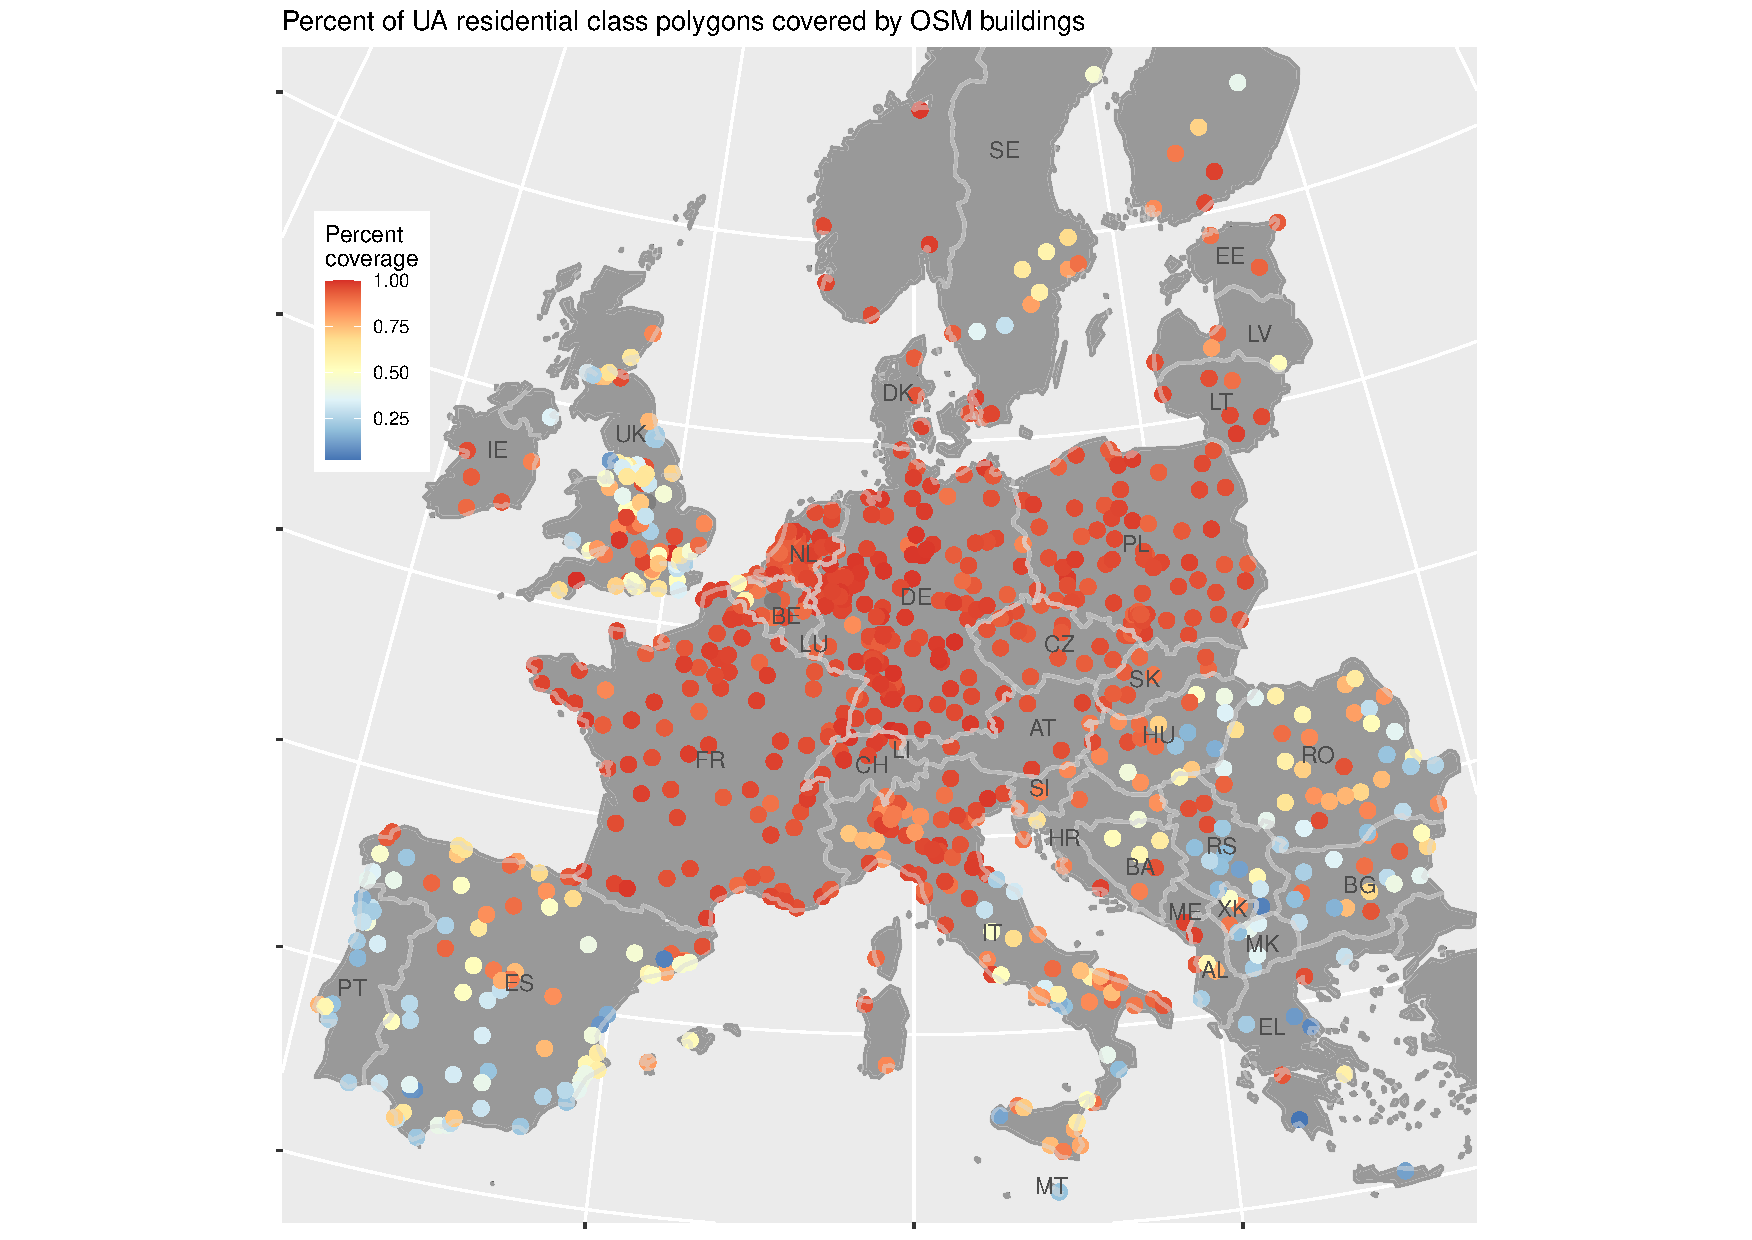
\includegraphics[width=1\textwidth]{2-1_osm_coverage.pdf}
\caption{Percentage of urban atlas residential class polygons (class 11100-11240) that contain at least one OpenStreetMap building polygon. Red colors represent a higher coverage - yellow and blue colors represent lower share of covered polygons.}
\label{fig:osmcov}
\end{figure*}

%Analysis to achieve Objective 1:
Our first objective was to develop a modeling approach that applies the Detour Index (DI) and Local Significance (LS) walkability indices.
For computational considerations, we limited the catchment area around each building to 500 meters network distance.
We calculated the Detour Index (DI) and the Local Significance (LS) index for each UGS inside the city core plus a buffer of 1 km.
We accounted for the maximum walking distance by calculating both indices for the residential buildings within a network distance of 500 m between a building entry and the nearest entry point of a UGS.

\textit{Detour Index (DI):}  The DI is an indicator of barriers in a network.
It accounts for the efficiency of the routes that residents take on their way to the nearest UGS \citep{Wolff.2021}. The DI combines the Euclidean distance, i.e. the direct connection between two points, with the network distance \citep{Esch.2014}:

\begin{equation}
\centering
\large{DI = \frac{D_{i,j}}{ND_{i,j}}}
\end{equation}

Where DI is the Detour Index, D is the Euclidean distance between points i and j, and ND is the network distance between the points i and j.
In the case of this analysis, the two points are the entry points of a residential building and the nearest entry point of a UGS.
The DI can assume values between 0 and 1.
A DI value of 1 represents a straight line between building entry and UGS entry, while a DI value closer to 0 means that the inhabitants of the building have to take a sub-optimal route to the nearest UGS.
If one building has access to several UGS within a network distance of 500 m, we decided to use the mean DI value.

\textit{Local Significance (LS):} The LS is usually used as an indicator of edge importance in a network analysis \citep{Esch.2014}.
We use a modified version from Wolff 2021 as an indicator of how many people have access to an UGS.
The LS also accounts for the size of an UGS as well as the distance between people’s homes and the UGS entries \citep{Wolff.2021}:

\begin{equation}
\centering
\large{LS = \frac{P_{i} * A_{j}}{ND^2_{i,j}}}
\end{equation}

Where LS is the Local Significance, p is the population of building i, A is the area of UGS j and ND is the network distance between the entry points of building i and UGS j.
This indicator can assume infinite values.
A higher population and area, as well as a lower network distance lead to higher LS values.
We attached the LS values to each segment (edge) of the path between building and UGS entries.
We summed the LS values of overlapping paths from multiple buildings, leading to higher values on higher frequented edges.
A more detailed summary on index building can be found in Appendix 3.

To demonstrate application possibilities of the indices, we visualized the DI and LS values for the area surrounding the Lene-Voigt-Park (LVP) in Leipzig.
The city of Leipzig is the largest city in Saxony, Germany. After a massive population loss in the 1990s, the city faced a major regrowth since 2012. Rising population numbers led to increased pressure on the open spaces of the city.
The LVP was a former train station area and has been out of use since 1942.
In the 2000s, it was converted to a public park and is fully open since 2004 \citep{Wolff.2017, StadtLeipzig.2022}.
Its diverse history and the population dynamic make the LVP an interesting test case for the demonstration of our results.
Since LS values tend to grow exponentially, we chose to use a logarithmic scale for visualization.

%Analysis to achieve Objective 2:
In our second objective, we wanted to compare the indices on a European level and assess in which cities the OSM data availability would facilitate our analysis.
%European comparison
For comparing the distribution of DI values in the European countries, we plotted the DI against the relative cumulative population in each city.
We aggregated the results to country level for easier visualization.
Furthermore, we mapped the percentage of people in a city that have a DI of 0.8 or higher.
To compare the LS values across European cities, we used the cities’ average of the summed LS values at the green space entries per UGS. 
%OSM data coverage
We assessed the OSM data coverage for 834 European cities.
We did so by computing the percentage of UA residential polygons that are covered by at least one OSM building polygon.
As a compromise, we used a threshold of 85\% OSM coverage (at least 85\% of the UA residential Polygons have to contain at least one OSM building polygon) for the comparison of our results across European cities.

%Analysis to achieve Objective 3:
The final objective was to implement the two indices we developed to demonstrate possible use cases for city planners.
To describe the impact of changes in different model parameters, we tested three different scenarios and calculated the change of the index values to the base model.

\textit{Alternative 1 – Unlimited access:} In the first scenario we demonstrated how the LS and DI indicators change if all barriers obstructing access to the LVP were removed.
To model unlimited access, we distributed hypothetical entry points every 5 meters on the network surrounding the LVP and applied the walkability indices to the changed conditions.

\textit{Alternative 2 – Green space development:} In the second scenario we investigated the impact of a development of the green spaces surrounding the LVP to residential buildings.
We assumed the following green spaces in the north of the LVP to be developed to high density residential buildings: Reudnitzer Park, Staphaniplatz, and the green space between Täubchenweg, Perthesstraße and Gerichtsweg.
To implement this scenario, we converted the former green space entry points to building entries.
We multiplied the size of the parks by the 95th percentile of the population per square meter value derived from the urban atlas high density residential class in the surrounding two kilometers.
We distributed the outcome uniformly across the former green space entries and applied the two walkability indices.

\textit{Alternative 3 – Population increase:} In the third scenario we modeled a population increase in the residential areas surrounding the LVP.
For each residential building in a distance of 2 km to the LVP, we increased the population value to the 95th percentile of the respective urban atlas residential class.
We then applied the DI and LS indices to the changed conditions.

\textit{Alternative 4 – Ensemble model:} In the final scenario we applied the changes from the unlimited access, the green space development and the population increase scenarios and gathered them in one ensemble model. 



\section{Results}

\begin{figure*}
\centering
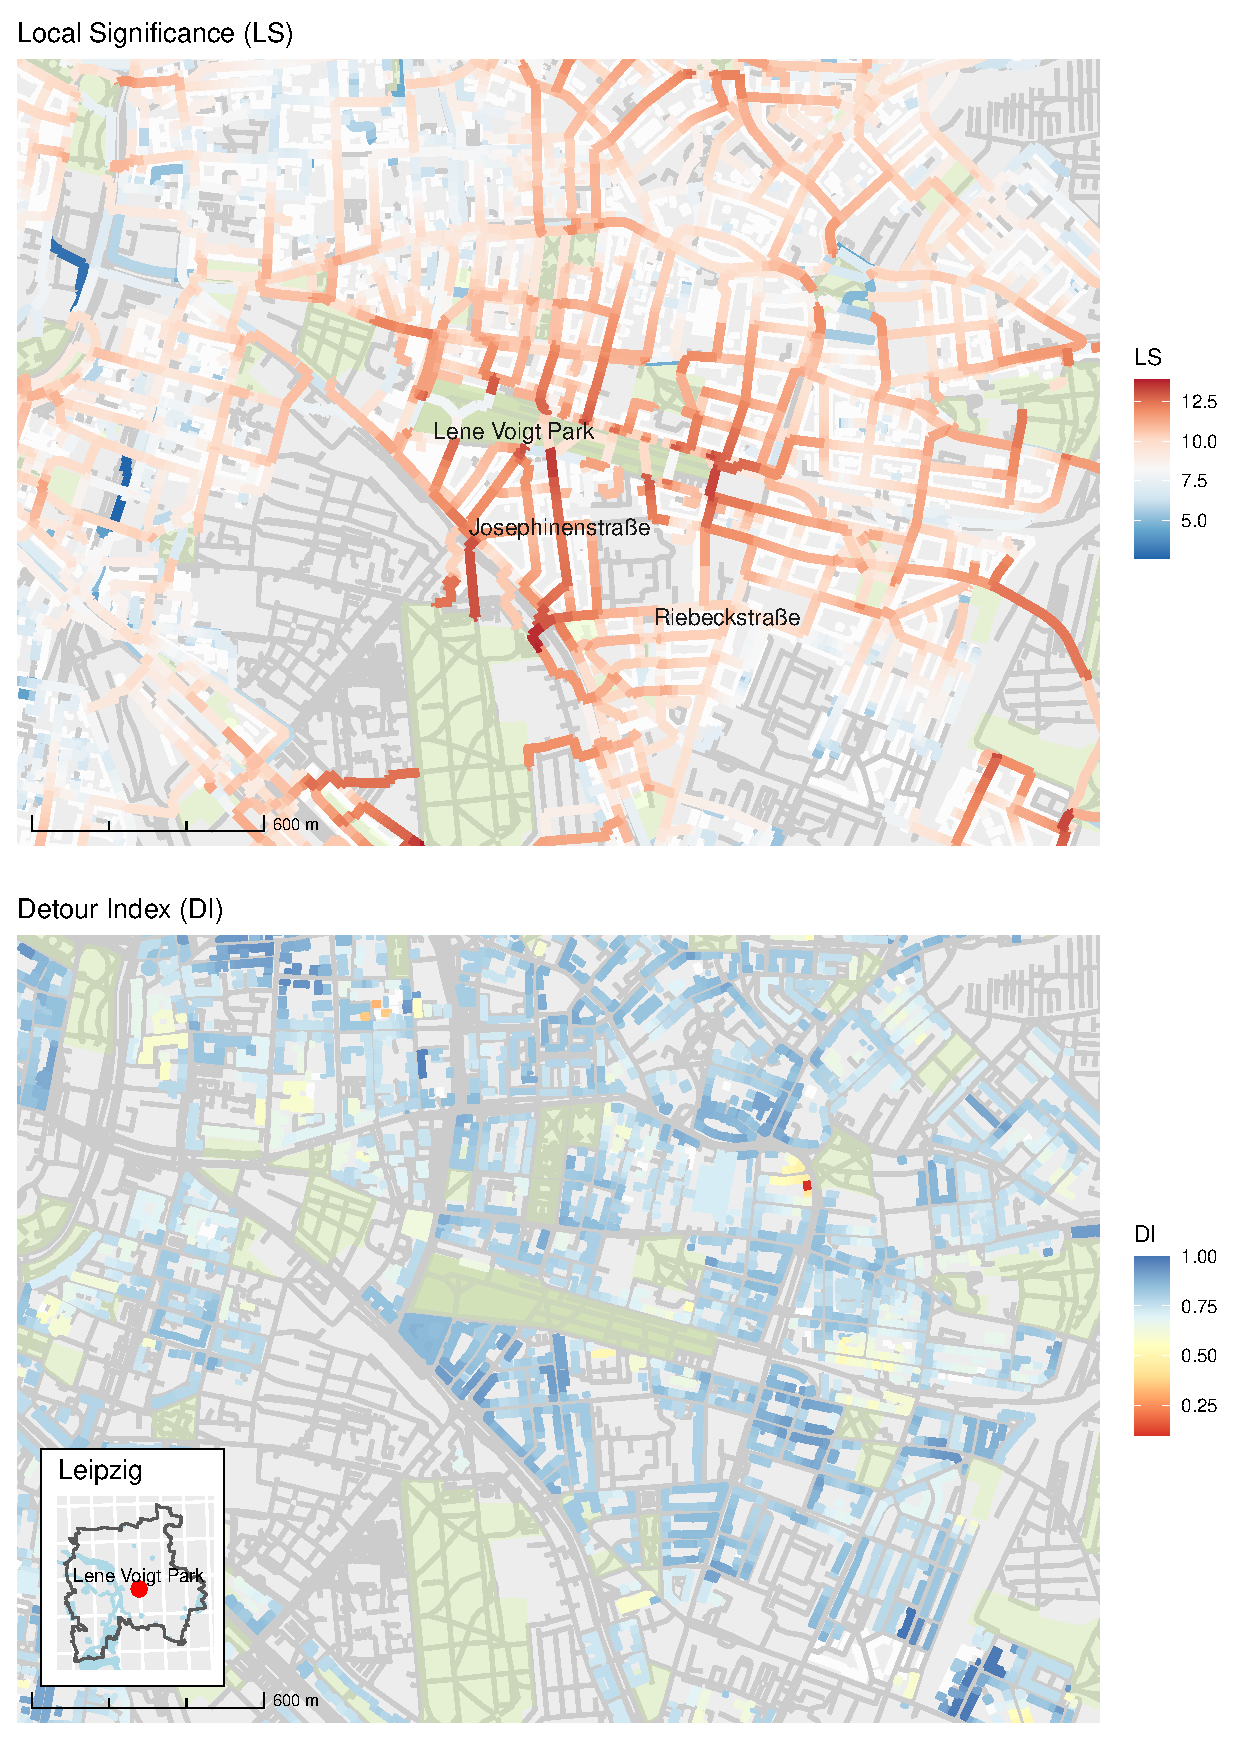
\includegraphics[width=.9\textwidth]{3-1_ls_di_plot.pdf}
\caption{The network colors depict the cumulative LS. A higher LS value is depicted by a darker red color, representing i.) more people taking this path, ii.) the people taking this path are living in closer proximity to the green space, and / or iii.) the path is leading to a larger green space. Since the LS values are cumulative, a higher value might also mean more paths from different buildings overlapping (See appendix 3 for further information). The building colors represent average DI calculated for all green spaces in a network distance of 500 meters from a building. The dark blue the color of a building is, the closer to one the DI value, the more direct can its residents travel to the closest green spaces. The opposite is the case if the color tends towards orange.}
\label{fig:lsdi}
\end{figure*}

\begin{figure*}[h!]
\centering
\begin{tabular}{llll}
\textbf{a) Vienna, Austria} & \textbf{b) Lisbon, Portugal} \\
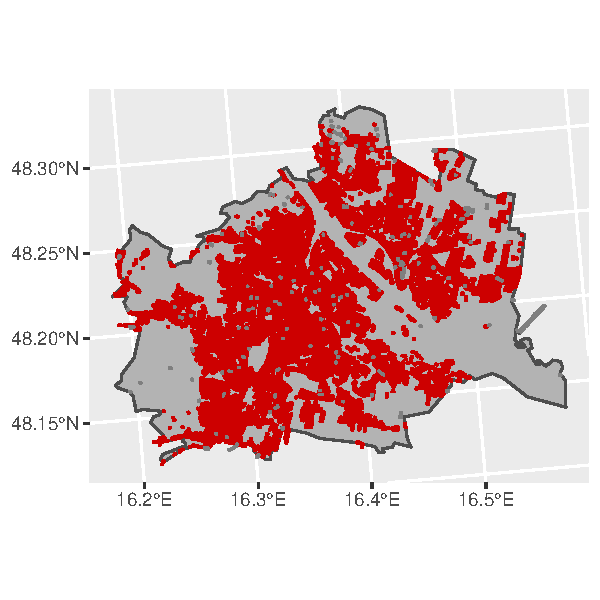
\includegraphics[width=.4\textwidth]{wien.pdf} & 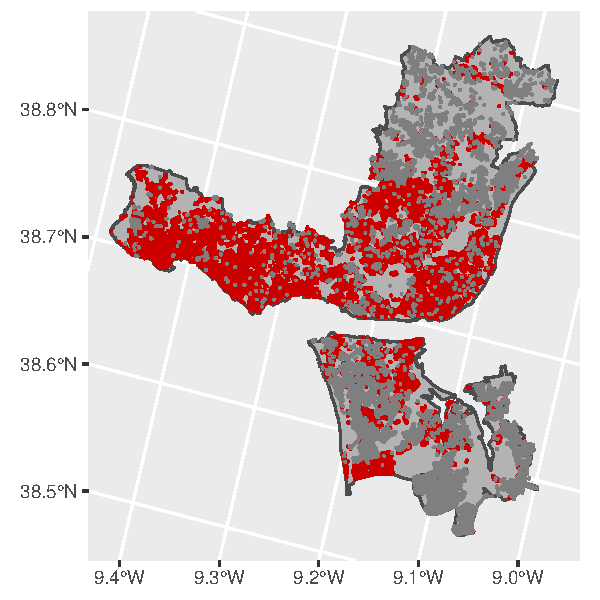
\includegraphics[width=.4\textwidth]{lissabon.pdf}
\end{tabular}
\caption{Urban atlas (UA) residential polygons covered by at least one OpenStreetMap (OSM) building polygon. Red: covered polygons; Darkgrey: not covered polygons.}
\label{fig:osmcovexample}
\end{figure*}

This study intended i.) to develop a modeling approach that applies the DI and LS walkability indices, ii.) to compare the results on a European scale, and iii.) to implement the indices by showing possible use cases for city planners.

\subsection{Applying walkability indices}
In this section, we present the results of applying the two walkability indices to the test case, the Lene Voigt Park (LVP) in Leipzig, Germany.
Figure \ref{fig:lsdi}a displays the local significance (LS) values that we calculated for the city of Leipzig, Germany.
The map shows the area east of the city center (top right corner of the map). 
In the center of the map, highlighted with a darker green, is located the LVP. 
Other green spaces are depicted in a lighter green, buildings and the network in white and gray, respectively.
Lower LS values are displayed in blue shades, higher values in red shades.

Due to the high density of green spaces and residential buildings in the area, an overall high level of LS values can be observed.
In general, LS values tend to grow towards green space entry points – i.e. higher LS values can be observed in closer distance to UGS.
Due to the cumulative nature of our LS representation, this effect symbolizes street segments with the potential for overcrowding.
Furthermore, high LS values are associated with direct connections between parks and residential buildings.
The highest LS values can be found at park entries adjacent to streets which connect UGS to areas with high population, indicating street segments that are highly visited for routes towards UGS. 
The eastern part of the LVP close to the Riebeckstraße is a good example for this (marker A on the map). 
Here, we find high LS values at those parts of the streets that lead to the residential areas in the north, east and south-east.
At the same time, we see that the Riebeckstraße in this area is actually a bridge with two Tram and two car lanes and few possibilities for crossing (see picture …). 
This circumstance is not represented in the street segment´s LS values.
Furthermore, the Josephinenstraße (marker B) which connects the center of the LVP to the next larger park in the south, the Friedenspark (marker C), displays high LS values.
On the other hand, we can make out lower LS values at streets with residential buildings that are close to the cut-off threshold of 500 meters distance to the nearest green space.
For example, in the southeast of the map, in many streets, the blue shade is getting brighter with each street segment until it switches over to red shades.
With each building entry, more inhabitants are expected to take these routes towards the nearest green space.
This increases the LS values of the street segments.

Figure \ref{fig:lsdi}b displays the detour index (DI) east of the city center of Leipzig.
Higher DI values are depicted in blue shades, lower ones in red shades.
High DI values can be found at buildings that are located at streets which lead directly to a green space entry. 
Along these streets there are straight formations of buildings with high DI values as can be seen in the south of the LVP. 
In contrast, there occur clusters of low DI values in areas where larger detours have to be taken to reach a park entry. Such areas can be found in the northeast of the map. 
Furthermore, we can observe low DI values at buildings that are close to several UGS but whose routes towards one or more UGS are inefficient.
Some buildings that are directly adjacent to one UGS, but have to take small detours to the nearest green space entry point, also show low DI values.
Lastly, we see that there are buildings close to UGS with high DI values but that have to cross larger streets or other obstacles to reach the green space entry point.

\subsection{Comparing walkability indices}
Here, we present the results of the OSM data coverage assessment and, later, compare the two walkability indices across Europe.
\ref{fig:osmcov} depicts the OSM coverage, i.e. the relative share of UA polygons that are covered by at least one OSM building polygon. 
Most cities in central Europe – in particular in Poland, the Czech Republic, Austria, Northern Italy, Switzerland, France, Belgium and the Netherlands – exhibit a very high OSM coverage of \textgreater 90\%. 
In the UK, northern Spain and the southeast of Europe, we see more cities with an OSM coverage of around 50\%.
In Portugal and the south of Spain few cities express an OSM coverage above 50\%, and most cities are around 25\% OSM coverage.
In \ref{fig:osmcovexample} we see two exemplary cities – Vienna as an example for a high OSM coverage and Lisbon as an example for a low OSM coverage.
The city of Vienna, Austria is a prime example for a high OSM coverage with 98.7\% of the UA residential building polygons covered by at least one OSM building.
A source of error explaining a fraction of the imperfect coverage in most cities are misclassified UA polygons (see Appendix 1b).
In another share of UA polygons, the population values might have been so small that none of the OSM buildings received a population count, so they got filtered out during the data cleaning process (see Appendix 2b).
In contrast, in Lisbon, Portugal 55.6\% of the UA polygons are covered by OSM buildings. 
As we see in \ref{fig:osmcovexample}, the OSM building coverage in Lisbon is declining with higher distance from the city center.
Further in the south of the city, OSM coverage tends to be more incomplete, as well.
Where OSM buildings are present, the workflow of generating LS and DI indices was still functional (see appendix 3).
On the other hand, large parts of the residential areas of Lisbon have no OSM coverage and, thus did not get index values.
This lack of DI values for a large part of the population would complicate a comparison with other cities that have a more complete coverage.
Also, comparing the LS values could prove unreliable, even though we use the average value at green space entry for the above analysis.
Missing residential buildings in the service area of green spaces would lead to LS values that might be lower than expected.
Due to these inconsistencies, we decided to exclude all cities with an OSM coverage of less than 85\% from our analysis.
Most of Europe’s capital cities feature a high OSM coverage and by choosing a threshold of 85\%, we only had to exclude 5 of them from our analysis (Lisbon, Athens, Budapest, London and Madrid).  

\begin{figure*}
\centering
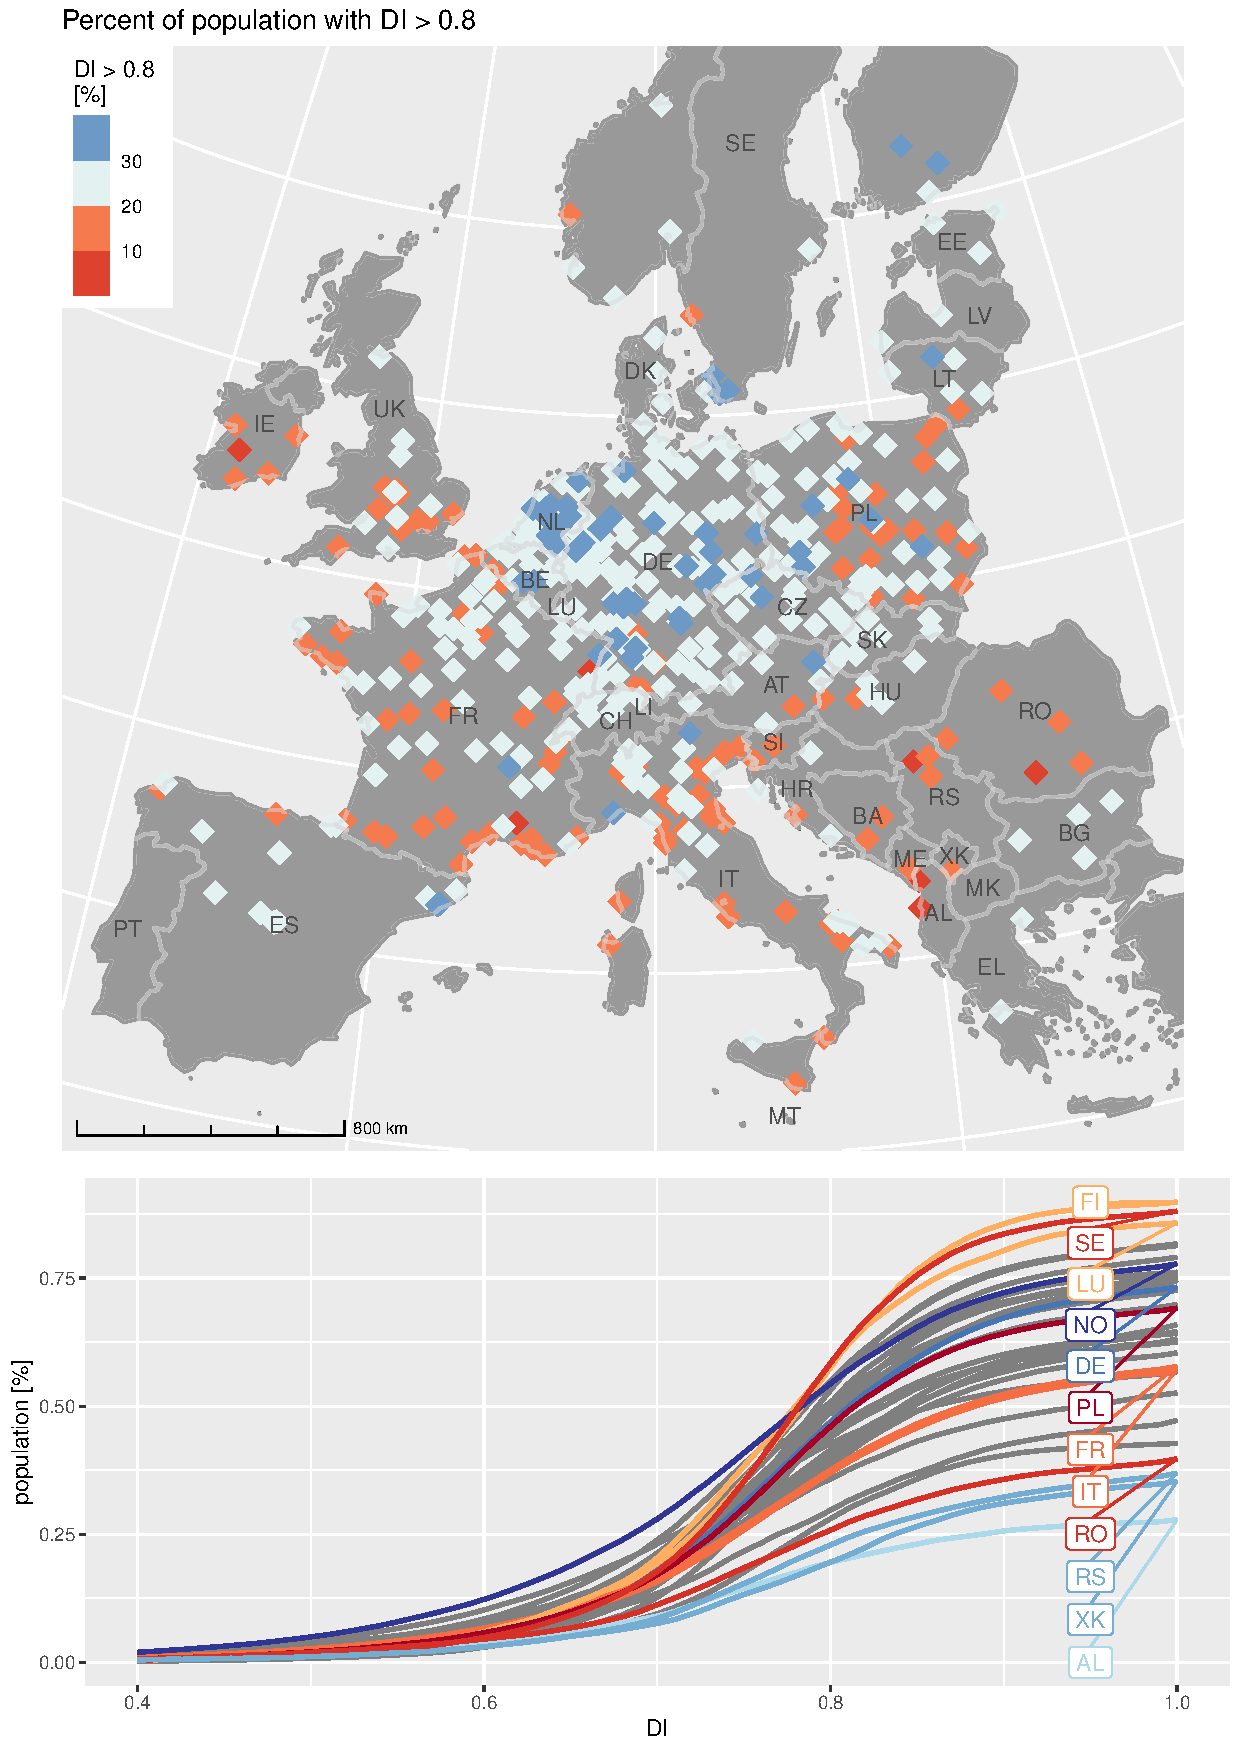
\includegraphics[width=.8\textwidth]{3-3a_di_map+plot.pdf}
\caption{Top: share of population with DI values of 0.8 or greater (in cities with OSM coverage \textgreater 85\%, n = 533). Bottom: DI values per share of population.}
\label{fig:dimap}
\end{figure*}


In this section we compare the DI and LS indices in 533 European cities with an OSM coverage of 85\% or higher (see previous section).
To compare the DI of European cities, we will have a look at the cities’ DI per relative cumulative population.
For the example of the LVP, a share of roughly 55\% of the population in the surrounding area has a DI of 0.8 or higher:
\begin{figure}[H]
\centering
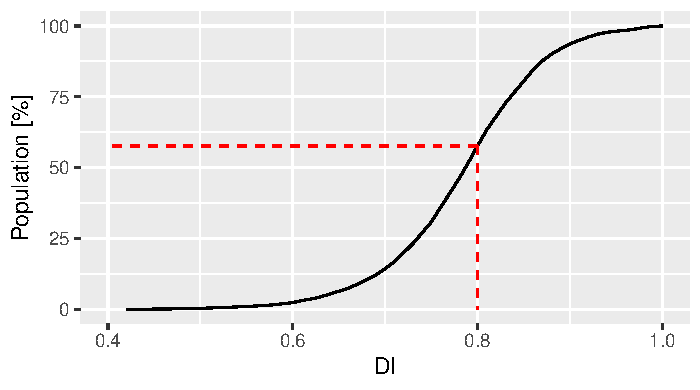
\includegraphics[width=.85\columnwidth]{3-2c_di_pop_lvp.pdf}
\end{figure}

In figure \ref{fig:dimap} we demonstrate this share of population for each city.
Here, we can observe a clustering of cities with mid- to high shares of population with DI values above 0.8 in northern and central European countries.
This cluster consists especially of cities in the Netherlands, Belgium and Germany, as well as the western parts of Poland and the Czech Republic.
In France, the UK, Italy and the eastern part of Poland, we see a larger share of cities with a lower percentage of population with DI values greater than 0.8.
Most Balkan countries, as well as Ireland have no cities with a \textgreater 20\% share of population in the highest DI segment.
As we can see in figur­­­­e x, the distribution of DI values plotted against the cumulative, relative population varies strongly across countries.
The ending points of the lines show the percentage of people with green spaces in a network distance of 500 meters. 
The slopes of the lines indicate how direct the inhabitants of a country can travel to the green spaces they have access to.
On the top end there are mostly northern and central European countries where more than 85\% of the urban population can reach green spaces in 500 meters network distance.
On the lower end there are mostly southern and south eastern European countries where less than 30\% of the population or less live in 500 meters network distance of green spaces.
It is notable, that on both ends of the spectrum, the sample size is limited to only a few cities (top: FI = 3, SE = 5, LU = 1, bottom: AL = 2, XK = 1, RS = 3, RO = 5).
Yet, there are countries with large city samples and a high percentage of population reaching green spaces in 500 meters network distance, like Germany (126 cities, 73\%) or Poland (68 cities, 69\%). 
Additionally, there are countries with large city samples and a lower percentage of people in proximity to green spaces like France (84 cities, 58\%) and Italy (56 cities, 57%).
In France, for example, we see a higher share of population with a more direct access to UGS in the north-eastern part of the country and a lower one towards the south-western part.
Generally, a curve that has a late onset and a steep slope means that more people have a more direct route to the nearest green spaces and vice versa. 
An example for this would be Finland, where about 32\% of the urban population have an DI of more than 0.8. 
On the contrary, the curve of Norway has an early onset and a lower ending point, resulting in a smaller share of people (23\%) having a DI in the highest 0.2 margin.

\begin{figure*}
\centering
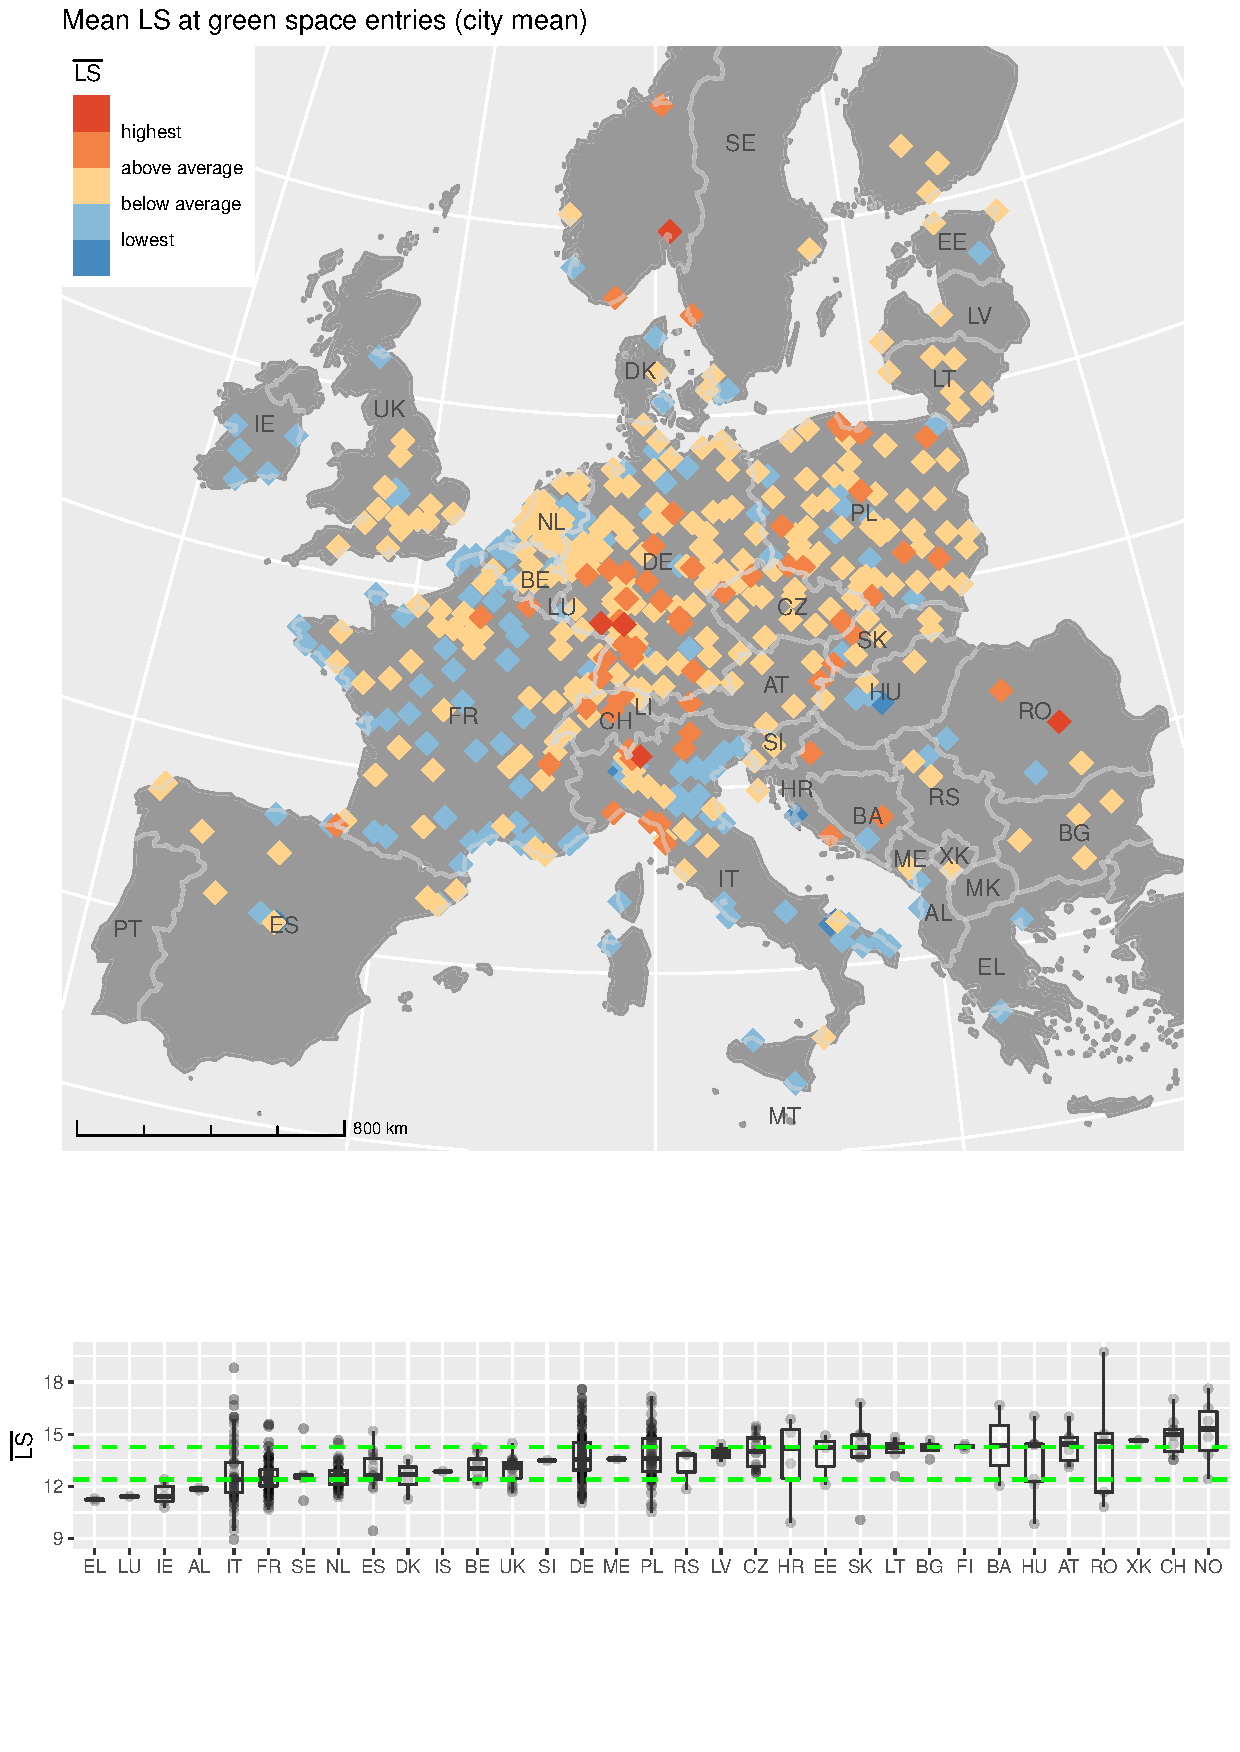
\includegraphics[width=1\textwidth, trim=0 150 0 0, clip]{3-3b_ls_map+plot.pdf}
\caption{Top: Mean LS at green space entry points per city (color) and LS coverage – i.e. percent green spaces in a city that have been reached by inhabitants (size). Bottom: Mean LS values at green space entry points per city. Aggregated by country.}
\label{fig:lsmap}
\end{figure*}

The average LS values at green space entry of the European cities also show a large variation.
For example, in \ref{fig:lsmap} we can observe above average LS values at the green space entries in mid- to southwestern Germany.
According to our results, in these areas the street segments at the UGS entries are highly visited, UGS are large and / or the population lives close to the UGS. 
In contrast, most of the cities in France or at the eastern coast of Italy feature rather low LS values.  
In Poland or the Netherlands, we find a mixed picture of cities with higher and lower LS values at green space entry.
In figure \ref{fig:lsmap} we see the LS values aggregated on a country level. 
Every point that is plotted behind the box-plots represents the average LS value at green space entry of one city.
Accordingly, we see that the differences in the number of cities where our analysis was feasible vary substantially between countries.
At the bottom and top ends of the chart, there are countries where relatively few cities are included in the final analysis, like Greece, Luxembourg or Norway.
From the countries with a larger share of cities that were eligible for our analysis, Italy has the largest spread of LS values.
Like France and the Netherlands, Italy’s mean LS at UGS entry is at the line indicating the lowest 25\% of cities, while the mean values of Germany and Poland are in the middle of the 25\% and the 75\% lines.
Again, a high average LS at UGS entry might indicate more people at the UGS entries, larger UGS and / or population living closer to UGS.


\subsection{Implementing walkability indices}
In this section we want to demonstrate how local planners can use the two walkability indicators that we applied before.
Therefore, we return to the example of the LVP as outlined in section 3.1.
We explore three potential alternatives in which we reshape the built environment as an expression of applied planning tools.
In each alternative, we alter one of the core variables that are used to calculate LS and DI.
In the first alternative, “unlimited access”, we assume that the LVP can be accessed from all around the park.
For the second alternative, “densification”, we selected a number of UGS north of the LVP and replaced them with residential buildings.
In the last alternative, “population growth”, we assume a certain increase in residents in the area surrounding the LVP.

\begin{figure*}
\centering
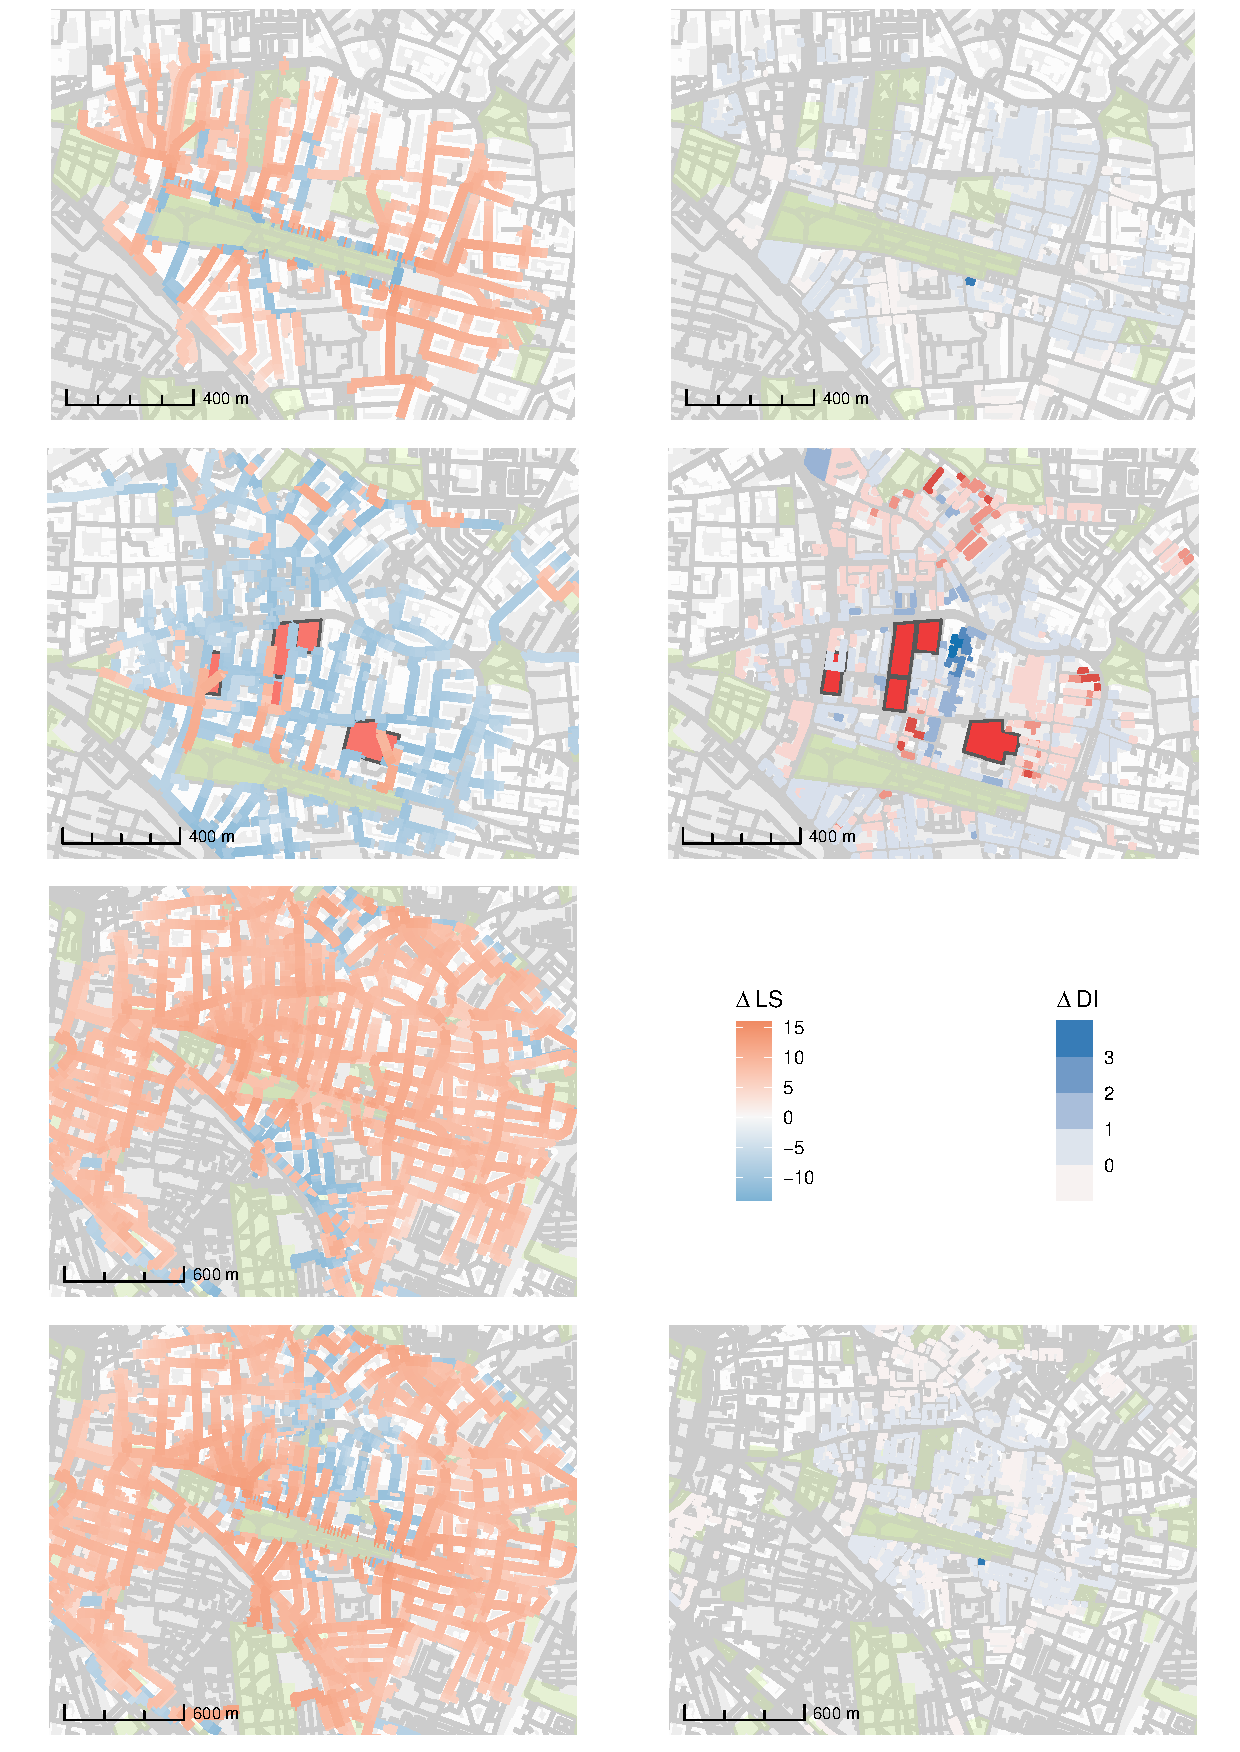
\includegraphics[width=.95\textwidth]{3-4_alternatives_plot.pdf}
\caption{Delta values for local significance (left) and detour index (right). Streets and buildings that expressed no change are not colored. An increased LS is mapped in red, a decrease in blue. Increasing LS values depict street segments that are higher visited. An increasing DI is mapped in blue, a decrease in red. Higher DI means that the trajectories from a building to the nearest UGS entry have become more efficient. The top two maps show the unlimited access alternative.}
\label{fig:alt}
\end{figure*}

\textit{Alternative 1 – Unlimited access:} In the first alternative, we demonstrate how the LS and DI indicators change if all barriers obstructing access to the Lene-Voigt-Park (LVP) were to be removed.
We do so by assuming a park entry every 5 meters on the network surrounding Lene-Voigt-Park.
As can be seen in figure \ref{fig:alt}a, a decrease in LS values occurs on all streets that are adjacent to the LVP. 
On most of the remaining streets, we observe an increased LS.
Thus, according to our model, removing the barriers along the edges of the LVP would result in less crowded streets surrounding the park, which may be a desirable effect for city planners.
On the other hand, more people could reach the LVP, increasing the overall amount of people traveling through net network and towards the park. 
Accordingly, removing entry barriers could also be a pull factor for an UGS.

Figure figure \ref{fig:alt}b shows the change of the DI values in the first alternative.
When the DI of a building increases, the routes towards the nearest UGS have become more direct, representing a facilitated access to the nearest UGS for the residents of the building.
Overall, we mostly observe minor changes of DI values (delta-DI < 0.1) when providing unlimited access.
We filtered out any delta-DI values that were smaller than +/-0.05 to place emphasis on the more significant changes.
It appears as though the change of DI values is mostly limited to buildings that are either very close to the park or that were not reachable before, but are now inside the threshold network distance of 500 meters.
A few buildings adjacent to the eastern part of the LVP express an increase larger than 10%. 
A larger area to the northeast and smaller areas to the east and south of the center of the LVP show a minor increase of DI values. 
These buildings may now be able to take a more efficient trajectory towards the LVP.
In the northwest of the map we see a cluster of buildings that seems to have gained access to the LVP via a direct path, which increased their DI values.
Contrary, in the southeast there is a couple of buildings that have gained access as well, but on a less direct path.
For these buildings the DI values decreases, meaning the average trajectories towards the nearest UGS have become less efficient.

\textit{Alternative 2 – Densification:} In the second alternative we intended to see how the indices behave if the green spaces in the city blocks north of the LVP were to be developed into residential areas.
To apply these changes, we switched the former park entries into building entries and distributed among them population according to the former park’s size.
figure \ref{fig:alt}c shows that overall, most of the LS values appear to decrease substantially. 
Since the UGS disappeared, the trajectories of the people that traveled to them have disappeared as well, leading to decreased LS.
Only on the paths connecting the newly built residential areas to the LVP and the former Johannes-cemetery in the west (marker A) can we see a substantial increase of LS values.
Overall, the reduction of the number of parks in the area seems to have a larger effect on the LS-index than the increase in population due to the newly “constructed” residential buildings. 

In figure \ref{fig:alt}e we see DI values mostly increasing in the area. 
Especially the buildings along the Heinrichstraße (marker B) that leads from the center of the LVP north experience a substantial DI increase.
Again, a higher DI means more efficient routes to the nearest parks.
Some areas in the east and north of the map express a decrease of DI values, representing less efficient trajectories towards the nearest UGS.
South and west of the LVP we observe a mixed picture of minor de- and increases.
The five green spaces that we intended to change into residential areas are comparatively small and, thus, “hard to reach”.
Taking them out of the equation seems to leave the surrounding buildings with more efficient trajectories towards the larger parks.

\textit{Alternative 3 – Population increase:} The third alternative is designed to demonstrate how a population increase would affect the DI and LS indices.
In this alternative, we assumed for each residential building a population increase to the 95th percentile of the population per area according to its urban atlas residential class.
Since we did not change the locations of any green spaces or building entries, the DI index did not change, either.
As we can see in figure \ref{fig:alt}e, the delta-LS is positive in the entire area.
In contrast to the other alternatives, changes are now scattered across the entire map, since we also applied the population growth all buildings in the area.
In this alternative, we see a similar pattern as in the basic LS map (see figure \ref{fig:lsdi}). 
LS tends to grow larger, the closer a street is to one of the large parks, specially along those streets, where the population flows from multiple areas combine on their way towards the UGS.
For example, we can observe high LS values between the LVP and the Friedenspark in the south of LVP.
The further away a street is from the larger parks, the lower the increase of the LS.
Close to LVP we now observe a large cluster with high LS values in the west.
If we have a look at the population data that is attached to the residential buildings, we can see that the area in the northwest of the LVP has several buildings with very high population (see appendix for larger version of the image).
Most of these buildings can reach the LVP only via the entry point at the northwest, which causes the high LS values in this area. 

\textit{Alternative 4 – Ensemble model:} In the final alternative, we applied all the changes of the previous three alternatives at once. 
The joint effects of removing barriers, developing the green space in the north and a population increase can be seen in figure \ref{fig:alt} f and g.
Figure \ref{fig:alt}f, shows that the change of the LS index is mostly influenced by the population increase and the green space development alternatives.
Due to the population increase, we see a general increase of LS, except for those streets that experience a decrease of LS due to the removed green spaces.
This makes the changes of the LS appear more diffuse than in the other alternatives.
Similar to the population increase alternative, we see a large area with high LS increase in the northwest of the LVP.
In this alternative we can simultaneously observe the effects of the population increase and the unlimited access alternatives.
The nearest entry point for the area with the high population residential buildings in the northwest has been shifted to the northernmost corner of the LVP in contrast to the third alternative.
As we can observe in figure \ref{fig:alt}g, change of DI is restricted to those buildings that either reached one of the now developed green spaces before or that can reach the LVP through one of the new entry points.
In the fourth alternative we can still see an overall increase in DI from removing the small and hard-to-reach green space in the north of the LVP.
Also, the mixed effects from removing the entry barriers to the LVP can still be observed in the south or the northwest of the LVP. 
For both, LS and DI, the overall changes in this alternative appear more gradual than e.g. in the densification scenario and are most apparent where we applied intense constructional changes.  



\section{Discussion}
In this paper, we developed a modeling approach that applies two walkability indices, the Local Significance (LS) and the Detour Index (DI) based on publicly available data and software tools \citep{EuropeanUnion.2020, RcoreTeam.2022, OpenStreetMapContributors.2020}.
We further demonstrated possible uses of LS and DI for city planners by using an urban park as a test case, the Lene Voigt Park in Leipzig.
In a final step, we compared the two indices for a set of European cities in order to detect variations between different cities. 
The application of our workflow was feasible, and the results were – with limitations – comparable on a European scale. 
In a consistent method reflection we report on the benefits and limits of the applied procedure.

%Applying indices
%LS
Wolff mapped the LS with colored straight lines that directly connect residential areas with the respective UGS. 
His representation of the index enables an overview of potential overcrowding in individual UGS and the strength of expected recreational flows towards the green spaces \citep{Wolff.2021}.
By plotting the LS in a cumulative way on individual street segments, we enable an even more targeted representation of the flows.
In an individual city, areas of high use intensity with potential for overcrowding can be identified at first glance as red clusters around the UGS’ in question.
Consequently, researchers and city planners can utilize our results to distinguish potential overcrowding effects that might limit accessibility of a specific UGS at individual street segments or green space entry points in order to display crowding effects of the corresponding Service Connecting Areas (SCA) \citep{Dworczyk.2021, Barthelemy.2018}. 

Our representation of the DI enables users at first glace to see which buildings have direct access to UGS, and weather they can reach UGS in and unobstructed manner. 
The index provides an estimation of potential detours people have to take in order to reach and UGS: the closer the route towards the UGS is to a straight line, the higher is the index DI suggesting a better accessibility. \citep{Esch.2014}. 
Consequently, this index is a good proxy showing discontinuous accessibility options of people without suggesting an artificial dichotomous differentiation between having and not-having access like indicated by fixed-distance buffers or isochrones. (e.g. \cite{Poelman.2018, Kabisch.2016}).
In some cases, the DI can be misleading, though. 
Low DI values may occur in close proximity to UGS as an artifact of small Euclidean and network distances values.
In these cases, a minor difference can lead to a low DI value even though the overall traveling distance to the next green space entry is relatively small.

Nonetheless, both walkability indices may be combined with local demographic, socioeconomic or environmental data, which can open up further opportunities for city planners.
For example, traffic, air pollution or -temperature or vegetation parameters along the street network might help in the decision process for intervention \citep{Poelman.2018}.

%Comparing indices 
Comparing the two walkability indices on a European scale has shown similar results as past studies.
The spatial patterns of high accessibility in central and northern Europe, and low accessibility in southern and eastern Europe, match those found in past studies.
For example, Kabisch found a lower UGS availability in south-eastern Europe within, both 300 and 500 meters \citep{Kabisch.2016}.
Poelman found similar results when using a proximity approach in 10 minutes walking distance for calculating a population weighted median of UGS area \citep{Poelman.2018}. 
Both studies enabled a spatial assessment of unequal distribution of UGS in a city, or between cities on a European scale.

%DI:
By comparing the relation of the DI and the cumulative population, we can add to these findings by showing potential barriers people have to overcome on their way to UGS.
Overall we could show a large variation across European countries.
While in southern and Eastern Europe, UGS availability in 500 meters network distance is comparatively low, the accessibility of the UGS seems to be low, as well.
In central and northern Europe, we observed not only high values of UGS availability, the routes people have to take to get there also seem relatively efficient. 
In countries with similar percentages of UGS accessibility like Norway and Germany the DI / population curve in figure \ref{fig:lsmap} depicts that a larger share of urban dwellers have a more direct path towards UGS in Germany, because here, the onset of the curve happens later.
On the other hand a late onset of the curve can result in an overall low accessibility, like in Italy,  while an early onset can still yield a relatively high accessibility as in Norway. 

%LS:
In comparing the average LS index values at UGS entries of the European cities, we found a cluster of cities with above average and high values in mid- to and south-western Germany.
Cortinovis et al found that European cities have shifted from a de-densification to a densification regime due to growth of urban population, decrease of land-take for residential use and higher immigration \citep{Cortinovis.2022}.
Furthermore, Wolff and Haase showed in their 2019 paper, that in southern Germany most cities express high residential density as well as only average supply of UGS \citep{Wolff.2019}.
High population pressure and short distances to or an unequal distribution of UGS might lead to relatively high visitation rates at green space entries.
These results confirm regional studies by Xu et al. from 2018 and 2020, who stated that a higher housing demand increases the pressure on GS availability \citep{Xu.2018, Xu.2020}.

%OSM coverage: 
Former studies relying on Urban Atlas (UA) were able to compare all 788 cities that are covered by this product in 2018 \citep{EuropeanUnion.2020}.
Enhancing the accuracy of the dataset by using OpenStreetMap (OSM) data has reduced the overall number of cities.
In this regard, we found a gradient of OSM coverage from north- and central Europe towards southern and south-eastern Europe.
Consequently, mostly central European cities exhibited a sufficient data coverage for effective comparison (Poland, Czech Republic, Austria, Northern Italy, Switzerland, France, Netherlands).
As long as the OpenStreetMap community is mostly active in central European countries, our approach is not really suited for a wholesome European comparison.
Due to the incomplete digitization of buildings in OSM it is mostly a central European comparison.
Furthermore, UA polygons that are covered by at least one OSM polygon is only a proxy for the potential coverage that may not yield inference about the nature and quality of the OSM data.
In data-scarce regions, the DI should be accurate for all buildings that are digitized in OSM and that are covered by the UA dataset.

%Implementing indices
To demonstrate potential applications for the two walkability indices for city planners and researchers, we implemented the LS and DI in three alternatives at our model case, the Lene Voigt Park LVP in Leipzig.
In general, we can say that an increase of the DI value of a building is a desirable effect because the residents have a more efficient – or more direct – way to UGS.
As a result, people might be incentivized to visit UGS more often and reap the positive effects of e.g. physical exercise or being in the nature \citep{Kabisch.2021}.
In contrast, an increase of the LS value of a street segment can usually be deemed negative. 
If no larger changes in the built-up structure have been implemented, an increasing LS means more people traveling through the same network, resulting in more crowded streets which might have an adverse effect on UGS accessibility.

The implementation of the LS and DI may not only help to assess green space demands of a city.
The two indices might also help city planners to test the effects of their actions regarding green and blue infrastructure on green space supply and demand before implementation. 
Additionally, the LS and DI may facilitate planning the street network, as well as residential units of an area together with the green and blue infrastructure, enabling synergies between departments and avoiding potential pitfalls.

%Alternative 1: Unlimited access
%LS: 
In the first implementation, we modeled an unlimited access to the LVP by adding green space entry points every 5 meters on the outline of the park.
At the immediate surrounding of the LVP, the LS index behaved as expected. 
Here, removing the entry barriers resulted in a decrease of the index, representing less crowding taking place, which is desirable for city planners, as it might alleviate the effects of overcrowding.
Nonetheless, the implementation of the unlimited access alternative showed ambiguous effects.
A UGS with less barriers might be more attractive, and thus, pull more people from the surrounding residential areas, resulting in more traffic in the remaining network and a higher overall visitation of the park itself.

%DI: 
The DI values of most of the residential buildings express only minor changes. 
The small changes of the network distance that occur when the nearest green space entry point is shifted do not carry as much weight if network and Euclidean distance values are larger.
In contrast, close to the LVP the small changes have a larger effect on the DI values, resulting mostly in substantial increases of the index.
The contradicting effects on the DI values of those buildings that have ‘gained’ access through removal of barriers show that considering the DI alone might not yield a full picture on UGS accessibility.

%Alternative 2: Densification
%LS: 
The LS index reacts strongly on the changes that we have applied to the built-up structure in the area during the second alternative.
Replacing the UGS with residential areas would cause the absolute number of people to use the network to increase. 
Our representation of the LS reacted contra-intuitively to the changes, though.
Removing the UGS reduced the overall number of trajectories modeled, which in turn decreased the index values for most of the network.
Only did the values increase at those street segments that lead from the converted UGS to the remaining ones.
The strong LS decrease in most of the network, as well as its evenly strong increase at certain streets highlight the importance of the UGS that were changed into residential buildings: Many neighboring residents can potentially use these places for recreation, while converting them and bringing even more people in will cause the remaining UGS to be more crowded.

%DI: 
Furthermore, the second alternative has shown that taking UGS that prove harder to reach out of the equation can increase the DI.
An increasing DI itself mean that residents travel along efficient trajectories towards UGS.
Thus, only considering DI values might implicate, that the green space accessibility for residents improves when green spaces are converted to build-up.
Since we are only looking at distances, the index lacks to account for an in- or decrease of the number of alternative green spaces.

Alternative two exemplifies one of the greatest weaknesses of our implementation of both indices: we merely account for the individual trajectories between residential buildings and green space entries without addressing the overall number of green spaces that are accessible per building. 
Consequently, our representation of LS and DI might still need further improvement in future studies to better represent the green space accessibility of urban dwellers.
At the same time, our analysis highlights an acute lack of research in this regard.

Alternative 3: Population increase
The modeled population increase in alternative three resulted in a general increase of LS values in the entire area. 
Where the population flows from multiple areas combine on their way towards the UGS we can visualize potential crowding effects that might occur if population increasing trends tend to continue \citep{Cortinovis.2022}.
These results also enrich different more areal-based approaches as on different density patterns emerging from the constellation of population trajectories and built-up area changes \citep{Wolff.2017}.

Alternative 4: Ensemble model
Finally, by uniting all changes, we see the complex interactions of built-up environment, population and UGS.
At the first glance, the population increase seems to dominate the other changes.
A closer look reveals the effects of converting the green spaces to residential area, as well as providing unlimited access to the LVP, though.
Overall, changing the build-up environment turns out to have higher impact on the flows of residents towards UGS than the population.
An increase in urban dwellers adds up to those crowding effects that are caused by other changes like in the densification alternative. 

%Limitations
There are several factors that limit out appraoch.
First, both indices are only as good as the data that they are built on. 
Errors in the UA or OSM data sets might propagate from data preparation to index building and multiply on the way. 
Both indices only account for the fastest routes from residential buildings to UGS in a walking distance of 500 meters, given the underlying network.
People might choose their routes towards UGS based on different factors than pure distance. Elements of attractiveness such as equipment, events etc. might encourage people to approach UGS in greater distances \citep{Biernacka.2018, Biernacka.2020}.
Our application of the LS and DI fails to account for obstacles people have to overcome on their ways to the nearest UGS like traffic lights, large streets or other physical barriers (see \cite{Barber.2021}). 
Another important point is, that, by using the urban atlas classes 14100 and 31000, we have only accounted for publicly accessible green spaces.
Furthermore, the role of private or residential green cannot be underestimated, since a high share of residents might prefer the use of their private green space over publicly accessible ones \citep{Chiesura.2004, Saumel.2021}.
This effect might cause the LS values to overestimate the flow of people from their homes to UGS.
By leaving private green out of the equation, we can not account for institutional barriers of accessibility \citep{Wolff.2021, Biernacka.2018}.
But combining the DI or LS with such measures might yield inference on a per building level instead of an UGS level, enabling quantitative and qualitative assessments with a higher accuracy than before (Biernacka et al. 2020). 
Lastly, reaching UGS by means of public transportation, private motorized transportation or cycling was not addressed by our study.
By including public transport into the model future research might remove further uncertainties of our approach.


\section{Conclusions}
%Conclusions:
In this study, we modeled the walkability of European cities – i.e. the quality of the routes people take to reach urban green spaces (UGS) – using publicly availability data and software. 
The Detour Index (DI) and Local Significance (LS) indicators that we employed not only enable small scale and high-resolution analysis of green space accessibility in single cities, but also allow for a large-scale comparison of cities and countries in Europe.
In adding to former research, we developed an approach for modeling the service connecting areas (SCA) between residents homes and UGS.
Instead of providing a dichotomous measure of having or not-having access to UGS, our approach enables inference about the SCA itself.
Nonetheless, in this study we only provide a broad overview – cities have grown over millennia and each data point in our graphs is an individual case study with challenges for itself. 
Therefore, it is important to make the results accessible and available (e.g. on a website) for urban planners so they will actually use them in their specific contexts.
Augmenting our results with environmental variables or other local data might enable researchers and city planners to better account for overcrowding effects and barriers that limit accessibility of UGS.

To enhance modeling of the walkability of a city in the future, we need to take the environment into account:
A more convenient walking experience on one street might cause people to change their trajectories and even take detours on their way towards UGS.
At the same time, a less pleasant walk may cause the opposite behavior.
Furthermore, certain features that are not reflected in the network we used, can turn out to be barriers for the accessibility of UGS, like large streets that have to be crossed.
Even though most of the data that is required to account for these features might be hard to get and to harmonize, an implementation can be easily realized by re-running our program, once the data is present.
Another point that the two indices are not sensitive for, is the fact that many residents have access to more than one UGS. 
Thus, building a new block of residential housing might not be as grave in a neighborhood with a plethora of alternative UGS. If the only park around is sealed and even more people are invited to live in the area, it can be a disadvantageous decision. 
A change of our index calculation process should account for UGS alternatives in future reasearch.
Since the two walkability indices are only an approximation of the potential flows, GPS data as is produced by companies like e.g. Google or Apple could facilitate a far more sophisticated analysis.
Especially overcrowding effects could be modeled with higher detail and even on a temporal scale. 
\bibliographystyle{apalike}
\bibliography{bibliography}
%\bibliographystyle{apalike}

\newpage


\begin{figure*}[ht!]
\centering
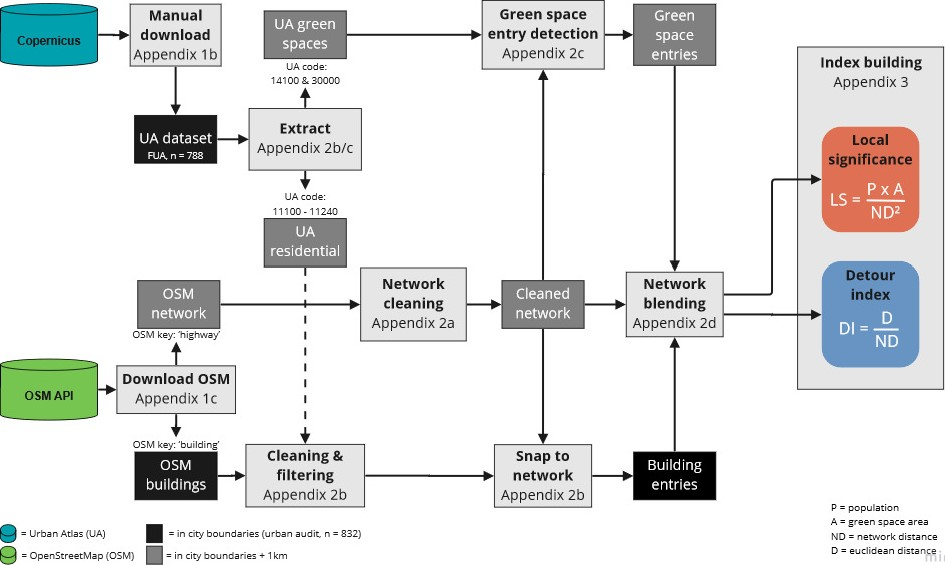
\includegraphics[width=1\textwidth]{5-appendix_flowchart_long.png}
\caption{Long version of the entire workflow: From data acquisition, to data preparation and index building.}
\label{fig:fc}
\end{figure*}

\section{Appendix}
In this section, we present all steps necessary to reproduce the results of the previous analysis.
We describe the data that we have acquired (Appendix 1), the pre-processing steps (Appendix 2) and the index-building steps (Appendix 3).

\subsection{Appendix 1 – Data acquisition}
Data acquisition is a crucial part of geographic analysis. Reliable sources of data are key in producing reliable output, so it is wise to carefully select one’s data sources \citep{vanderMeer.2019}. To model the walkable environment of cities on a European level, we chose to create the Local Significance (LS) and Detour Index (ID) \citep{Esch.2014, Wolff.2021}. For the creation of the LS and DI on a European scale, we require data on i.) green spaces, their entry points and their area, ii.) residential buildings, their entry points and the number of residents inhabiting them, and iii.) the network that connects the residential buildings with the green spaces. Finding comparable data for a Europe-wide study can be a challenge in itself. There is a plethora of network, building and green space data provided on national or municipal levels. They are provided in different formats and quality and have different access restrictions. Gathering these data, city by city or country by country could potentially create a comprehensive source of data for our analysis. But overcoming all restriction barriers, finding comparable data, bringing all of the different formats into alignment would prove too difficult for this work. For the purpose of developing the workflow to create LS and DI for European cities, we have chosen to acquire Urban Atlas (UA) and OpenStreetMap (OSM) data. UA and OSM are both freely accessible and offer more or less comparable data on a European scale. We derive the green space data as well as the information on the city’s inhabitants from UA. From OSM we derive the network and the buildings. We estimate the locations of building and park entry points based on both datasets (see Appendix 2b and 2c). This chapter shows the measures we have taken to find and access data that covers as much of our area of interest as possible.


\subsubsection{Appendix 1a – City boundaries}
In order to facilitate the analysis of the service connecting areas in European cities, we need a spatial delimitation of the target cities. Urban Atlas data is mostly available for the functional urban areas (FUA) of the cities. But as described in the chapter before, the extent of the FUA can vary from large commuting zones to city cores. To be able to compare European cities in this analysis, we need a harmonized dataset of city boundaries. For this purpose, we chose to use the urban audit city administrative units \citep{EuropeanUnion.2020, UrbanAudit.2022}.


\subsubsection{Appendix 1b - Download urban atlas (UA) data}
%Why UA?
For constructing the Local Significance index, we require reliable population estimates.
UA provides exactly this with a minimum mapping unit of 0.25 ha, which turns out to be a 	convenient resolution of mostly city block level. 	
Furthermore, we can use UA data to implement another safety net for filtering the 	OpenStreetMap buildings.
%The UA data / Copernicus
UA provides high-resolution urban land use data with a minimal mapping unit of 0.25 ha and 27 land use classes. The latest version of UA maps the 2018 urban land use of 788 European cities with more than 50.000 inhabitants according to the Functional Urban Area (FUA) as determined by the DG Regional and Urban Policy of the European Commission.  With version v13, the UA data from 2018 has received its latest update and received population estimates for each polygon. UA is mostly based on Earth Observation data and is backed by other reference data, like commercial data, OpenStreetMap data or topographic maps. Input data is automatically classified and validated afterwards. Thematic accuracy of the urban land use product is stated to be >85%, positional accuracy < +/- 5 meters \citep{EuropeanUnion2020}.

%Downloading the data / pitfalls
Copernicus, the data provider of UA does not offer an API for downloading the data required. Consequently, we either have to use the Copernicus web page to manually download the data for each city, or we use the interface to select all cities at once and, thus, create a download request. This process requires a registration for the Copernicus web page. Also, we 	can only download the latest version of the UA data \citep{EuropeanUnion.2020}.

\begin{table*}[]
\resizebox{1\textwidth}{!}{%
\begin{tabular}{lllll}
\hline
source              & version                     & coverage           & data                                                                     & specifics                                  \\ \hline
Urban Audit         & 2020                        & 832 cities, Europe & city boundaries                                                          & urban kernel                               \\
OpenStreetMap (OSM) & download: April -  May 2022 & global             & residential buildings                                                    & key: 'building’                            \\
                    &                             &                    & network                                                                  & key: 'highway’                             \\
Urban Atlas (UA)    & 2018 v13                    & 788 FUAs, Europe   & urban green spaces                                                       & classes: 14100, 31000                      \\
                    &                             &                    & \begin{tabular}[c]{@{}l@{}}residential areas  \\ Population\end{tabular} & classes: 11100, 11210, 11220, 11230, 11240
\end{tabular}%
}
\caption{Data overview table}
\label{tab:overview}
\end{table*}

\subsubsection{Appendix 1c – Download OpenStreetMap (OSM) data}
%Why OSM?
For the analysis of the walkable environment of European cities, we needed available and comparable data on the network that connects the residential buildings with the public green spaces.
To ensure a high resolution of the analysis, we needed data on the residential buildings, as well.
OSM offers global coverage with varying data density. 
Fortunately, the reliability of OSM data is usually higher in larger cities.
Since we wanted to develop a workflow using free and open source data that produces comparable results for all of Europe, OSM was the only available choice.

%The OSM project:
OSM is a community-based project that provides free geospatial data.
The OSM community seeks to create a database of the entire planet that is free and editable.
For creation and verification of the OSM map, the community uses a wide variety of data sources. 
Among these sources are aerial photographs, GPS-devices and maps.
The OSM community consists of a variety of contributors, ranging from enthusiastic mappers to GIS-professionals and engineers.
Registration is mandatory for editing the OSM map (\url{https://www.openstreetmap.org/about}).
At the time of writing this paper, the number of registered OSM users is about 8.5 million. (\url{https://planet.openstreetmap.org/statistics/data_stats.html}).
In 2022, the entire OSM dataset contains a total of roughly 7.7 billion nodes and about 860 million ways.
OSM follows an “open data” policy, meaning that the data can be used for any purpose, as long as OSM and its contributors are mentioned (\url{https://www.openstreetmap.org/about}).

%Downloading OSM data:
Downloading larger chunks of OSM data can prove difficult. 
For downloading OSM data, the OSM community offers the Overpass API on different public instances (\url{https://wiki.openstreetmap.org/wiki/Overpass_API}).
Since OSM is an open source project, all servers that provide OSM data are considered public goods.
Heavy usage of the Overpass API has to be avoided and should not surpass 10.000 requests per day or 1 GB download volume (\url{https://dev.overpass-api.de/overpass-doc/en/preface/commons.html}).
If over-use of the servers is detected, a user will usually be timed out (\url{https://dev.overpass-api.de/overpass-doc/en/preface/commons.html}).
To download OSM data in accordance to the community guidelines, we created a R package that automatizes downloading OpenStreetMap network and building data on a city level (\url{https://www.github.com/blabohm/MA/}).

%Functionality:
The downloading-workflow consists of the download\_OSM function and various sub-functions and relies heavily on the osmdata package \citep{Padgham.2022}.
Required input for the download-OSM function is the city code (URAU-code) of the desired city and the directory containing the file with the city boundaries.
The workflow follows the steps: a) subdividing the city, b) downloading the data, c) cleaning the data and d) writing the data to file.

\textit{a) Subdividing the city:} We have taken several precautions to limit the number of requests and the overall download size of each request. 
As a first measure, the download\_OSM function extracts the city boundary that corresponds to the provided URAU-code.
The city boundary will be cut into a grid of boundary boxes with 2 km edge length.
Larger sized boundary boxes have shown to produce too large data chunks. 
Especially in dense parts of large cities these large data chunks led to queries that were frequently canceled by the Overpass API.
Smaller boundary boxes, on the other hand, created an unnecessarily high number of queries.  
A smaller edge length of the boundary boxes would also cause more duplicates on the edges of the boxes.

\textit{b) Downloading process:} During the downloading process, R will try to download the OSM data for each of the boundary boxes individually.
For each of the boundary boxes, R will communicate with the different instances of the Overpass API.
If each instance offers the same number of slots, one will be chosen randomly.
Otherwise, R will choose (one of) the Overpass API instances with the highest number of available slots.
If no slots are available, R will timeout for 30 seconds and restart communication with the Overpass API afterwards.
The chosen Overpass API instance will be set via the set\_overpass\_url- function from the osmdata package.
In the next step, R will create an overpass-query using the osmdata opq-function.
R will create individual queries for the building and the network data, i.e. create two separate download requests.
With the created queries, R will try to download the OSM data that is located inside the boundary box from the set Overpass API instance.

\textit{c) Cleaning the data:} Once the OSM data is downloaded to the computers RAM, R will try to ensure the integrity of the data.
First, only the columns matching the string “building\$” (for buildings) or “highway” (for network data) will be selected. 
Previous attempts have shown that several non UTF-8 characters in the column names of the OSM data are not compatible with the Geopackage (.gpkg) format.
In the second cleaning step, R will cast the geometries to polygons (for buildings) or linestrings (for network data).
The OSM data is provided in individual layers for each geometry class (point, linestring, polygon, multilinestring, multipolygon).
This step will first and foremost ensure the data’s compatibility across different R packages and functions.
In addition to the compatibility, casting the geometries to a lower level will also prevent erroneous geometries from causing trouble down the workflow.
OSM is a large and diverse dataset with only the community validating the correctness of the data - so errors have to be expected.

\textit{d) Writing the data to file:} Finally, R will generate an output directory based on the input directory and the city code.
If the OSM data consisted of multiple layers with different geometry classes, the now homogenized data will be appended to the same file and the same layer.
These steps will be repeated until the OSM data in each boundary box is downloaded.
The individual subfunctions that are being called by the download\_OSM function can be called separately by a skilled user, as well. 


\subsection{Appendix 2 – Data preparation}
%Why data preparation?
Real world data is unfortunately almost never ready to use.
To ensure a certain amount of consistency in our analysis, we have to make sure that data is cleaned, i.e. erroneous or duplicated data is fixed or removed.
In addition to cleaning, we also have to bring the data into the right format for our later analysis.
For creating the Detour Index (DI) and Local Significance (LS) index, data preparation will encompass the steps i.) network preparation, ii.) building preparation, iii.) green space entry detection and iv.) network blending.
We have gathered these steps in the data preparation workflow.

\subsubsection{Appendix 2a – Network cleaning}
%Why network cleaning?
OpenStreetMap (OSM) is a large and heterogeneous dataset that is being audited by the OSM community.
Unfortunately, the immense amount of data and heterogeneity of the OSM contributors are a guarantee that the data is not ready to use.
In cleaning the network prior to taking further steps in the analysis, we ensure a higher consistency of the results.
%Network cleaning
A variety of errors can cause problems when using network data for an analysis. 
One common error in network data is small deviations in the coordinates of lines that are supposed to be connected.
It often occurs that the coordinates that make up the endpoint of the first line and the starting point of the next line are almost the same.
If the point coordinates that make up the lines are stored with too much precision, a small deviation between these two points, can cause the lines to be found unconnected by our analysis tools.
Other common mistakes are duplicated nodes or crossing lines that have no common node at the intersection and are thus not connected.
On top of the usual pitfalls of working with network data, we have downloaded city-wide data in tiles of 2×2 km. 
Prior to the analysis, these tiles have to be joined together to create a network covering the entire city.
On the edges of these tiles, there may be overlapping paths due to e.g. a street crossing through the border of one of our tiles.
The overlapping part of the street would be downloaded twice in the two adjacent tiles.
For a consistent analysis, we have to make sure that most of these errors are being detected and corrected.
This task is being carried out by the networkPrep function of our script.
%Functionality
The cleaning process is made up of the networkPrep function, which itself relies on a plethora of different sub-functions.
The networkPrep function takes as input i.) the city code in URAU format, ii.) an input directory containing the required layer with the city boundaries and the network tiles that were downloaded by the download\_OSM function and iii.) an output directory for saving the output.
The directories containing the required input can be set manually or will be guessed automatically from the in- and output directories.
The network cleaning process follows these steps: a) spatial and thematic filtering, b) combining the network tiles and c) cleaning the network:

\textit{a ) Spatial and thematic filtering:} The first step of the network cleaning process involves loading the city boundary that is corresponding to the URAU code that was provided to the networkPrep function. 
Since we downloaded the OSM data in rectangular boundary boxes, we downloaded a ‘surplus’ of data at the tiles overlapping the edges of the city.
The city boundary will later be used to spatially filter out all information that is located outside of the city.
Thus, the amount of data that is stored on the machine will be reduced.
On loading the city boundary, the networkPrep function will also apply a buffer of 1000 meters to the boundary.
The buffer ensures that the cleaned network will later cover areas outside the cities border that households living at this border can visit inside a 500 meters walking distance.
In the next step, the networkPrep function will list all tiles that have been downloaded and whose names match the cities URAU code.
During this process, the boundary file will be transformed into a well-known-text (WKT) filter.
The WKT filter will be used to load only those parts of the downloaded OSM data from file that are needed because they are located inside the city boundaries.
In addition to spatially filtering the OSM data, the script will automatically discern the highway column in the OSM data from the many other columns that contain the string ‘highway’.
The highway column contains the information describing the importance of the path in the network (e.g. motorway, primary street, residential road etc.).
All path with the value ‘motorway’ in the highway column will be filtered out (\url{https://wiki.openstreetmap.org/wiki/Key:highway}).
Motorway was the only value that we could consistently identify as the only class of network elements to be accessible only for cars and not for pedestrians. 
For example, filtering out primary roads, even though they are supposed to ‘often link larger towns’, led to missing important walking axis that are accessible to pedestrians in large German cities.

\textit{b) Combining network tiles:} Now the actual network combination process starts. 
After spatially and thematically filtering the network data, it will be casted to linestring geometries.
This way we make sure that no other geometry types will cause errors in the further analysis.
The pre-cleaned network tiles will now be written into the same layer of a Geopackage file.
Appending the individual tiles to the same layer of one file has proven the most efficient way of combining the network tiles.
Other ways of combination would include loading all network data into the RAM of the machine and combining it there, taking a larger amount of time.
After all files of downloaded OSM network data are written to disk, the network data is ready for further cleaning steps.

\textit{c) Cleaning the network:} In the last part of the network cleaning workflow, the actual pitfalls of network data are being tackled.
The network cleaning script heavily relies on the tidygraph and the sfnetworks R-packages and loosely follows the sfnetworks pre-processing and cleaning tutorial by Lucas van der Meer, Lorena Abad, Andrea Gilardi and Robin Lovelace (\url{https://luukvdmeer.github.io/sfnetworks/articles/sfn02_preprocess_clean.html}).
Further cleaning of the network dataset involves i.) removing double entries, ii.) rounding coordinates, iii.) subdividing edges, iv.) spatial smoothing, v.) removing unconnected edges and vi.) removing overlapping edges.

i.) Removing double entries: In the first cleaning step, all double entries in the now combined network dataset are being removed. This process uses the dplyr ‘distinct’ function which only removes double entries from the data frame without touching the geometries of the data. In this step there will not be removed any overlapping edges, yet.

ii.) Rounding coordinates: Now we make sure all coordinates that make up the lines of the network data are exactly the same where lines are supposed to be connected. For this correction, we chose to reduce the precision of the network data. We did so by applying a rounding function to the coordinates of the line geometries. This process will implement a minor imprecision of a few centimeters in the network data.  And too much rounding can cause lines of zero length which will cause errors in later analyses.
Subdividing edges: In the later analysis, we rely on the sfnetworks package. When creating a network from OSM network data with this package, the linestrings of which the network consists will make up the edges. The endpoints of these edges become the nodes of the network. Edges that share the same endpoint also share the same node – i.e. they are connected. An edge can still have interior points that define its shape but are not nodes of the network. If an edge shares exactly the same interior point with another edge but this point is not a node, they are not being considered connected in the network structure. To rule out any unconnected edges due to this error, we can split the overlapping edges at their common point. This point, in turn, becomes a node of the network and the edges are connected. The function to\_spatial\_subdivision of the sfnetworks package in combination with the tidygraph function convert does exactly this. All edges are be connected at shared interior nodes. Edges will not be connected if they are overlapping but do not have any shared nodes, reducing the danger of connecting bridges to the paths that are lying beneath them.

iii.) Spatial smoothing: A spatial network might as well contain nodes that do not play any connecting role in the network structure. These nodes have only one incoming and one outgoing edge. These pseudo nodes would only increase the complexity of further analysis and, thus, increase the time it takes to compute the results. To remove pseudo nodes, the sfnetworks package offers the function to\_spatial\_smooth, which can be used with the tidygraph function convert. After removing a pseudo node, to\_spatial\_smooth will transform the two adjacent linestring geometries into a single edge. 
Removing unconnected edges: Another common pitfall in the downloaded OSM network data are unconnected edges that form their own network structure. Edges can be unconnected from the rest of the network due to several reasons. They can, for example belong to paths that are located inside of a courtyard or atrium that has no publicly available connection the rest of the network. Leaving unconnected edges in the network dataset would in the later analysis cause unreachable areas of the city. E.g. residential building entries could be assumed to be located in these areas and thus vanish from the analysis. To counteract this source of errors, we filter the network data using the tidygraph group\_components function, which groups a network by its connected components. We use this function to keep only those edges that are connected to the largest component – i.e. the city network. 

iv.) Removing overlapping edges: In the last step, we aim to remove any edges that are still overlapping from the network. An overlap could, for example, be an artifact of downloading the OSM network data in 2x2 km tiles. If a street is crossing the boundary between two of the tiles, part of it might be downloaded once for each tile. Downloading the street twice will result in two longer edges with ending parts that are overlapping. Overlapping edges would cause the same path to appear multiple times in the network. This could potentially cause the local significance index values, which are supposed to accumulate on the edges, to distribute across several overlapping edges. For removing overlapping edges, we have devised the remove\_overlap function. Remove\_overlap relies on the R- package sf and its st\_covers function. To remove overlapping edges, remove\_overlap will separate the network into those edges that cover multiple other edges and edges that only cover themselves. Consecutively, it will split the edges that are covering other edges and only keep those parts that form a unique spatial feature.


\subsubsection{Appendix 2b – Building preparation}
%Why building preparation?
To create the Detour Index (DI) and the Local Significance (LS) index, we are only interested in the residential buildings.
By downloading all buildings from OpenStreetMap (OSM) that are located inside a certain area, we have also downloaded buildings with non-residential function, though.
In addition to filtering out non-residential buildings, we need population data attached to buildings to calculate the LS values.
These tasks will be executed during the building preparation process.
%Building preparation
During the process of downloading the building data from the Overpass-API, we retrieved a plethora of polygons representing all buildings in a city.
Attached to the building data there is often some information on the building type or use. 
Since the OSM contributors that create the building data have different levels of experience and different motivations, the annotation of these information is rather inconsistent, so we cannot solely rely on it.
To circumvent the inconsistent annotation, we will compare the OSM buildings with the urban atlas (UA) data that we have downloaded manually.
UA land-use data provides information on residential areas of cities on a European level.
We can utilize the information on residential areas to filter out all OSM buildings that are located outside of these areas.
This way we try to retrieve all residential buildings of a city.
A side-effect of this procedure is, that we can in the same step join the population data that is contained in the UA dataset to the OSM buildings.
Information on the population is mandatory for calculating the LS index.   
For further steps in the analysis it is also required, that we proceed with the centroids of the buildings, rather than the polygons.
We have bundled these tasks in the buildingPrep function of our data preparation workflow.

%Functionality
The building preparation process is integrated in the buildingPrep function in our R-program.
The buildingPrep function takes as input i.) the city code in URAU format of the city that should be prepared, ii.) an input directory containing the layer with city boundaries, the downloaded OSM buildings, the directory containing the UA data and iii.) and output directory for writing the ready-to-use building layer to disk.
All directories containing the required input will be guessed automatically from the input directory.
If desired, individual file names can be specified.
The process of building preparation follows these steps: a) loading UA data, b) filtering OSM data, c) adding population values, d) adding building ID, e) calculating building centroids.

\textit{Loading UA data:} The UA dataset usually encompasses and area larger than the city core. To reduce this dataset and, thus, saving disk space and computation time, we reduce it to the city outline. For the reduction of the UA dataset, we first load the city boundary with the corresponding URAU code from our layer with all European cities. When loading the UA data from file, the city boundary will be converted to a well-known-text (WKT) filter. With the WKT filter we will only load UA data into the machines memory that is located inside the city’s boundaries. Consecutively, the UA data will be filtered so only the residential classes (11100, 11210, 11220, 11230, 11240, 11300) and the columns that are necessary for later steps will be left (population, identifier and class code). The UA dataset is now ready for the further building preparation.

\textit{Filtering OSM data:} The OSM building data that we downloaded from the Overpass API are stored in 2x2 km tiles. Like with the network data, there will be a surplus of data in those tiles that are overlapping the city boundary. Upon loading the individual OSM building tiles into the machine’s memory, we use a WKT filter similar to the one we used before to keep only entries that are located inside the city’s boundary. In the following steps, invalid and empty geometries will be filtered out and the geometries will be cast to polygons. These steps have proven necessary to prevent broken geometries from causing errors in later processing steps. Also, splitting multipolygons that are potentially still contained in the dataset into their respective parts has proven to reduce errors in the later workflow. In a further filtering step, we execute a spatial join to attach the UA residential data to the OSM buildings. All buildings that have no UA data joined to them can now be filtered out. In the last OSM filtering step, we make use of the information that is stored in the OSM data. For a fraction of the building data, the ‘building’ column contains information on the use or function of a building. Usually the value is merely ‘Yes’ or ‘NA’, but some for larger, non-residential buildings there is often a descriptive character string in here. On gathering the unique values of the building column from the OSM data of several cities, we could make out a list of words that could safely be excluded. We use this information to exclude buildings tagged with the following strings: "\^ mall\$", "train\_station", "garages", "hospital", "parking", "sports\_centre", "university", "gas\_station", "school", "hall", "government", "prison", "sports\_hall", carport", "garbage", "waste". After taking these filtering steps, we made sure to mostly use residential buildings in the further analysis.

\textit{Adding population values:} To later generate LS index values, it is necessary to add a population count to every residential building. In the first approach, we add the UA population to the OSM building via the respective size of the buildings. In this process, we sum up all building areas in each UA polygon and distribute the population values according to a building’s share of the total building area. This approach follows the assumption that buildings inside a UA polygon – which mostly represents a city block that is delimited by streets or other uses – have homogenous structure and population per area. After the first approach of adding population to the OSM buildings, we need to rule out one further error source. A fraction of the residential polygons in the UA dataset has not been assigned population values. To nonetheless add a population-count to the buildings that are located inside these polygons, we distribute population according to the average population value per building area for each UA residential class. Eventually, we remove all buildings that have not yet received a population value.  

\textit{Adding building ID:} To be able to link the index values of the future analysis back to the building polygons, we create in an intermediate step an individual building-ID for each polygon. This is done by adding an incremental number to each building polygon in each UA residential polygon. The filtered building polygons will now be stored to file for later use. 
 
\textit{Calculating building centroids:} Finally, to facilitate the integration of the building data into the network analysis, we transform the polygons into their respective centroids. For this step we decided to use the st\_point\_on\_surface function from the sf package, rather than a function taking a geometric centroid. The centroid of all points that make up a geometry can fall outside of the initial geometry. Since we want to use the resulting points to later estimate building entries, a point outside the initial geometry would be undesirable. The thus filtered building centroids will be written to file for use in the later analysis.

\subsubsection{Appendix 2c – Green space entry detection}
%Why green space entry detection?
To measure the distance from a building entry to the nearest green space, we need a fixed point that demarcates the nearest entry point to that green space.
Unfortunately, the data that we have acquired does not provide reliable information on those entry points.
Consequently, we have to estimate where the entry points of each park in a city might be located on a network.

%Green space entry detection
To detect green space entry points as reliable as possible, we chose to intersect the urban atlas (UA) polygons of the classes urban green (14100) and forest (31000) with the OpenStreetMap (OSM) network data.
We used the outline of the UA polygons so the intersection algorithm only yields points that are on the edge between green space and city.
During the data preparation workflow, the greenSpacePrep function in R will take on this task.
When detecting green space entry points, the greenSpacePrep function will apply increasing buffer sizes until each green space in a city has at least one entry point.  
Furthermore, we have to account for inhabitants that live at the edges of poly-nuclear cities and are thus able to travel to green spaces across city borders.
To avoid this problem, we have to integrate the UA green spaces of adjacent cities into the analysis.

%Validation
To refine the approach of green space entry detection, we used the outlines of green space polygons with buffers of different sizes applied to them.
We selected three Berlin green spaces to validate the accuracy of the different buffer sizes.
To cover a large variety of urban green spaces with the available work force, we chose the Tempelhofer Feld, the Viktoriapark and the Treptower Park.
In the Viktoriapark, park entries are well defined by surrounding walls / greenery.
The Treptower Park is rather open and has lots of meadows at its edges.
Furthermore, the Treptower Park is delimited by the river Spree on its northern side and a train station at its western end.
The former airport Tempelhofer Feld is in the original UA data set classified as ‘sports and leisure facilities’ but fulfills in our opinion the function of an urban green space.
The Tempelhofer Feld is delimited entirely by a fence.
Entry is only possible at gates that are designated for public entry.
At each of the three sites, we recorded the GPS coordinates of each entry point. 
We tried to mark the locations where people are expected to enter the green spaces, e.g. paths leading into a park, gates, bridges or station exits.
We used the resulting GPS points to estimate how much over- or underestimation was produced by automatically detecting green space entry points with the different buffer sizes. 
To account for the different buffer sizes, we manually selected edges from the OSM network data demarcating possible entry trajectories into the green space for each GPS point.
We used Google Earth Pro aerial photographs and QGIS to mark the network paths serving as entrance trajectories.
The different buffer sizes around the green space polygons we tested are: -10, -5, 0, 5 and 10 meters.
For the following sensitivity analysis of the different buffer sizes, we checked for each validation trajectory whether or not it was detected with the utilized buffer size.
‘Detection’ in this case means that the ‘detected’ park entry was inside a buffer of 1 meter around the validation trajectory.
We measured the accuracy of a buffer size by assessing if green space entries were correctly detected (validation data) without producing pseudo entries (e.g. at intersections with the street network that are no entry points).
We calculated the highest producer accuracy for the buffer sizes of negative 5 meters and 0 meters.
This means that the algorithm was equally good at detecting true positive green space entries with both buffer sizes.
The commission error was lowest for negative 5 meters and increased in both directions.
So when applying a lower of higher buffer, the algorithm falsely detected green space entries that were not in the validation data.
High producer accuracy and low commission error resulted in the highest overall accuracy for a buffer size of a negative 5 m around the green space polygons.
The second most accurate buffer size was a buffer of 0 meters. 
With increasing buffer size, the accuracy of the detected park entries decreased and the overestimation of park entries increased further.
A possible explanation for this outcome might be that most of the green space polygons align with the nearest larger streets.
A negative buffer will in this case better detect the paths that are emerging from these streets.
Of cause, these results have to be taken with a grain of salt, since we only validated them in Berlin and only with a handful of green spaces.
There is by far no guarantee, that these findings can be readily translated to other cities or countries.
When looking into the outcome, this should always be considered.

%Functionality
In the data preparation workflow that we wrote in R, the greenSpacePrep function will assign at least one entry point to each green space of a city.
The greenSpacePrep function takes as input i.) the city code in URAU format of the respective city, ii.) the input directory that contains the city boundaries layer and the UA and network data, and iii.) an output directory for storing the resulting green space entry points.
The paths to the required input files will be guessed automatically but can be provided manually, as well.
The greenSpacePrep function follows the steps a.) checking the proximity to other cities, b.) loading the UA green space from all cities in question, c.) detecting green space entry points and d.) rounding the geometries and outputting the data:

\textit{a) Checking proximity to other cities:} When checking the proximity to other cities, we start by loading the target city boundary from the city boundaries layer that corresponds to the URAU that we used as input. After loading, we will apply a buffer of 1000 meters to the city boundary. This way we make sure that any green spaces that are inside a network distance of 500 meters from any residential buildings in the city will be factored in later. Now we will check if there are any other cities from the layer with all city boundaries intersecting with the buffered city boundary. We do this again by first converting the buffered city boundary to a well-known-text filter (WKT). The WKT filter is then used to extract the functional urban area (FUA) code from any other city that intersects with the target city boundary. We use the FUA code here, because the UA file names are encoded in this style. Several URAU coded cities can share a single FUA code. If any neighboring cities were detected, the respective FUA codes will be passed on the next function. Otherwise, we will proceed with only the URAU code of the target city.

\textit{b) Loading UA green spaces:} When loading the UA green space data, we initially filter the directory with all UA city data for the directories matching the city codes (URAU and / or FUA) that were passed on from the previous function. Upon iterating through the respective UA data directories, we use a WKT filter representing the buffered target city boundary to load only the UA data into the machines memory that is located inside the target city. To further reduce the data size, we select the columns containing the FUA code, the UA class code, the UA identifier and the area, i.e. the size of the polygon. We filter the resulting data to obtain polygons identified with the UA classes 14100 or 31000. If a future user desires to use UA data from 2006, be wary of the fact that the forest code in 2006 was 30000. Furthermore, any further areas that are desired to be taken into account in the following analysis can be added here. For example, we have manually added the Tempelhofer Feld in Berlin, because it is classified as ‘sports and leisure facility’ in UA. We consider the Tempelhofer Feld to fulfill the same role as an urban green space, though. The resulting green spaces are gathered in a temporary file and passed on to the next function. On request, an output directory can be provided.

\textit{c) Detecting green space entry points:} When detecting the green space entry points in a city, we first load the respective network data that we have cleaned during the network cleaning process. Now we apply the negative 5 meter buffer to the UA green spaces that we obtained in the previous step. To prevent any geometry errors during the further analysis, it is advisable to make sure all green space polygons are of the correct geometry type (Polygon). In the next step we cast the negatively buffered green space polygons to linestring geometries. This way we retrieve the outlines of the green spaces which we can now intersect with the network data. Some green spaces might be to far from the next network edge or by chance their outlines did not intersect with the network. To make sure all green spaces receive at least one entry point, we check if there are any green spaces left without. We iteratively increase the buffer size in steps of 5 meters, intersect the remaining outlines with the network and check again. To reduce computation time, we increase the steps to 10 meter for a buffer size between 50 and 100 meters, 25 meters for buffer sizes between 100 and 200 meters and 50 meters for buffer sizes larger than 200 meters. When no green space is left without an entry point, we pass the result on to the next step.

\textit{d) Rounding geometries:} Before writing the green space entries that we detected in the previous process to file, we round their geometries. This has proven to prevent R from randomly crashing during the further analysis. If not provided by the user, the greenSpacePrep will automatically generate an output file name and store the green space entries here for further use. 

\subsubsection{Appendix 2d – Network blending}

%Why network blending?
After all data was acquired, and all necessary data cleaning, filtering and conversion steps have been carried out, we need to bring the data together.
For the creation of the Detour Index (DI) and Local Significance (LS) indices, we need to produce one dataset that contains all network information and one dataset that contains the residential building and park entry points.
Additionally, these two datasets have to be harmonized to enable routing operations that are necessary for index creation.
We carry out these tasks during the network blending workflow.

%Network blending
To calculate the DI and LS indices, we require on the one hand information on the locations of the residential buildings and green space entry points.
One the other hand we need a network that connects the two.
In the previous data preparation steps, we have carried out all tasks to acquire and process these data.
Yet, we have three individual datasets that have no connections whatsoever.
The network structure that we use for our analysis consists of edges and nodes. 
Each edge is a line that connects a start and an end node.
A node can have several edges emerging from it.
Two edges are connected, if they share the same node.
Each node will be given an index number in addition to its coordinates.
In turn, an edge will receive the index numbers of its start and end nodes. 
Consequently, to facilitate network analysis with the data that we have acquired and prepared so far, we need to integrate the entry points of the residential buildings and the green spaces into the network.
Each line of the network data will be an edge in the network structure with nodes representing the starting and ending points.
Additionally, the building or green space entry points that have no relation to the network yet have to become nodes in the network structure, as well.
To integrate buildings and green space entry points into the network, for every point we have to i.) find the nearest point on the closest network edge, ii.) split the edge at that location and iii.) add a new node to the network.
The newly created node will receive all information from the original point and the index numbers of both, nodes and edges will be updated.
The creators of the R package sfnetworks utilize for this process the metaphor of throwing the data into a blender and mixing them together.
For blending points into a network, they have developed the st\_network\_blend function.
In our network blending workflow, we rely on the st\_network\_blend, as well as other functions from the sfnetworks package.

%Functionality
We have bundled the steps necessary to execute the network blending process in the networkBlend function.
The networkBlend function takes as input i.) the city code of the target city, ii.) an input directory containing the layer with the city boundaries, and iii.) the output directory of the previous data preparation steps containing the network data, the residential building entry points and the green space entry points.
The output directory will be used for storing the results of the network blending process as well.
The individual paths to the layers containing the output of the previous data preparation steps will be created automatically based on the output directory.
If desired, the paths can be set manually as well.
During the network blending process, we will follow the steps a.) dividing the data into grid cells, b.) snapping and blending the green space and residential building points data into the network, and finally c.) combining the grid cells back together:

\textit{a) Dividing the data into grid cells:} In the network blending process, we carry out a couple of computationally very intensive tasks. Especially the process of snapping a great number of points to a large network can use lots of resources. To increase the overall speed with which these tasks are being solved, we split the dataset into smaller chunks and distribute the work across multiple computation cores. These cores can now process the tasks in parallel, instead of having to perform them in series. By splitting the data, we not only save computation time by distributing the data, but we also greatly speed up the snapping process. Snapping means that a point is being ‘moved’ to the nearest point on the nearest line. If we reduce the size of the network, the snapping algorithm, instead of having to search the entire city network for the nearest edge, only has to search the reduced dataset. We parallelize the network blending process by overlaying the city boundary layer with a 2x2 km grid and keeping only those grid cells that intersect with the city boundary itself. The resulting grid cells, we pass on to the next function.

\textit{b) Snapping and blending the green space and residential building points into the network:} To run the computation for each grid cell from the previous function in parallel, we use the R packages foreach and doParallel. By default, the process will run on roughly 75\% of all available computational core that the machine has available. Increasing this value could render the machine incapable of executing other tasks, which can lead to unexpected crashes, or, if run on a shared device (e.g. a server) spark social conflict. In the snapping and blending process, we convert the respective grid cell into a well-known-text filter (WKT). We now use the WKT filter to consecutively load the building and green space entry points and the network data that is located inside the grid cell into the machine’s memory. We load the network with a buffer of 100 meters, so any points that lie close to the grid cells edge have a change to be snapped to a street that is in the next grid cell. In a consecutive step, we merge the future nodes that should be blended into the network (i.e. the building and green space entry points) into a simple feature (sf) object. Now we hand the sf object containing all entry points and the network data that is inside the grid tile to the blending process. During the blending process, we utilize the sfnetworks R package. Particularly we use the as\_sfnetwork and the st\_network\_blend functions. The former converts the network data that is located inside the respective tile into a sf-network. A sf-network is a combination of the sf data structure with the igraph data structure. In a sf-network, the edges and the nodes are stored with their respective data in two separate data frames but belong to the same object. The as\_sfnetwork function converts the network data into a sf-network by converting each linestring geometry of the network into an edge of the sf-network and by adding nodes at every starting an ending point, as well as adding the required index numbers. The st\_network\_blend function now takes this network and the sf object with all the point geometries and blends them together. In short, the st\_network\_blend function entails:

i.) checking if a point geometry is located on an edge 

ii.) if not: snapping the point to the nearest location on the nearest edge 

iii.) and either: if the location is not already an existing node, splitting the edge and integrating the new node into the sf-network

iv.) or: attaching the points data to the existing node

A more elaborate and detailed description of the process can be found here: (\url{https://luukvdmeer.github.io/sfnetworks/articles/sfn03_join_filter.html#}). This method comes with a couple of drawbacks, though. If there are multiple points that share the same node location, only the first point will be used in the final sf-network. The same counts for a point having multiple possible locations on nearby edges. And lastly, the blending process can cause precision errors, where a node that is intended to represent the starting or ending point of an edge is a tiny distance away from the edges end point. This happens due to internal rounding errors in R and causes two connected edges not to be recognized as connected. To prevent this from happening, we have set the tolerance parameter of the st\_network\_blend function to 1 mm. After the blending process is complete, we write the resulting tiled sf-network into a temporary file, where it waits for further processing. As mentioned in the past paragraph, this process takes place in parallel for each tile of the city grid. So, we end up with several individual two files per grid cell. One file containing the edges and one containing the nodes. 
\textit{c) Combining the grid cells back together:} After snapping and blending the points of the residential buildings and green space entries to the network, we end up with several files containing edges and nodes. For the network analysis, one file containing all edges and one containing all building and green space entry nodes of the city. Combining the nodes is rather simple. We consecutively read all individual files containing the nodes and make sure all geometries are correct. Afterwards, we assign all columns the correct data type to make sure they can be merged together and append all files into the same geopackage database. The combination process of the edge files has to consider that edges can cross borders of grid cells, so we are likely to have created duplicated edges close to the borders. To remove these duplicates, we utilize the st\_network\_join function of the sfnetworks R package. The st\_network\_join function performs a join of the network data, making sure duplicates are removed to a minimum. Nonetheless, we utilize the remove\_overlap function from the network cleaning data preparation step to further reduce the number of overlaps. Using redundant functions in this step has proven to enhance the quality of the network that we later use for the network analysis. In a final step, we also write the combined edges to their geopackage database and delete the tiled edge and node data to reduce disk usage.
At this point data preparation is finished. The required data that we need to create the indices is cleaned and in the right format to serve as input into the network analysis.



\subsubsection{Appendix 3 – Index building}

%Why index building?
Now that all data necessary to create the Local Significance (LS) and Detour Index (DI) indices is ready to use, we can start calculating the two indices for the entire city.
The indices will be built on the city level during our index building workflow.

%Index building
In the process of index building, we want to calculate the DI for each building and the LS for each street segment.
To facilitate the creation of the two indices, we need to find the green space entry point that is closest to the respective residential building.
For calculating the DI for one building and the nearest green space entry, we need to measure the Euclidean distance and the network distance between the two points.
Consequently, we calculate the average DI for all green spaces that have an entry point located in a network distance of 500 meters of less.
The LS index also requires the network distance.
Additionally, we need the population of the residential building and the size of the park to calculate the LS.
We attach the LS value to each edge (i.e. each street segment) that is crossed on the way from the building entry and the green space entry. 
Similar to the DI, we calculate the LS for each green space that can be reached in a network distance of 500 meters or less.
Finally, for each edge we sum up all LS values of all routes from each building to the respective green spaces.
This way we end up with one cumulative LS value for each edge in a city.

%Functionality
We have integrated the process of building the LS and DI indices into the getIndices function of our index building workflow.
The getIndices function takes as input a working directory that contains the previously created databases containing the nodes and edges data, as well as the file with the building polygons.
All paths can be handed manually to the getIndices function or will be created automatically based on the working directory.
By default, the output will be written to the working directory if not specified otherwise.
The index creation workflow follows these steps: a) listing the green space identifiers, b) inputting the data, c) calculating and saving the indices and d) joining the index values back to the network and buildings:

\textit{a) Listing the green space identifiers:} Creating the indices is a computationally intensive process. Particularly the process called routing (i.e. finding the fastest route between two points in a network) can use lots of resources. To increase the speed of completing the LS and DI computation for an entire city and to speed up each computation itself, we use a number of methods. First, we use the UA identifiers that come with the UA data to facilitate parallelization of the process. During the previous steps we have kept these identifiers together with the green space entry points. By iterating through the object identifiers of the green spaces, we can distribute the computation across multiple computational cores. Similar to the snapping and blending process in the previous chapter, our function uses 75\% of the available computation cores. Setting this number higher might not be recommended under certain circumstances. The green space identifiers are now used to set up the parallel processing.

\textit{b) Inputting the data:} When we set up parallel processing in R on a Windows machine, we have to account for certain limitations. If run on Windows, each task that we hand to R to compute in parallel will start a new Windows process. Unfortunately, this means that we have to input all of our data separately into each of the processes, which can take up lots of memory. Particularly loading the spatial data into each process has to be planned meticulously to not overwhelm the machines memory and cause (not so) unforeseen crashes. On iterating through the green space identifiers, we first load the green space entries that are associated with the identifier via a SQL query from the nodes database directly into the memory. We then apply a buffer of the 500 meters distance (that we have chosen as a cutoff value) to the green space entries and convert them into a well-known-text (WKT) filter. The WKT filter we use to directly load only those building entries from the nodes dataset into memory that are needed for creating the DI and LS indices in a network distance of 500 meters from the green space entries. Similarly, we use the WKT to load the network data that is located inside the buffered area from the edges database. The data we have obtained for the analysis now is not yet a real representation of the 500 meters network distance, but a severe reduction of memory used. With all data necessary to calculate both, the DI and the LS indices for a single park, we can now proceed with the process.

\textit{c) Calculating and saving the indices:} In the first step, we generate an origin-destination cost-matrix to find the nearest green space entry point for each building entry. Secondly, we compute the Euclidean distance and the shortest paths between each pair of building and green space entry points. From the shortest paths, we can easily add the network distance to each path by summing up the lengths of each edge that the path encounters. At this point, we use the network distance to filter out buildings that are located further away than 500 meters from any of the green space entries. After these steps we have acquired all parameters necessary to calculate both indices: The population is attached to the building nodes as well as the network and the Euclidean distances. The size of the green space is attached to the green space entry nodes. After calculating the DI values for each building, we write the index values with their respective building IDs (see Appendix 2b) to a simple csv-file. Consequently, we write the LS values and their respective edge IDs (see Appendix 2a) to another csv-file. To save disk space, we strip the output of all spatial data. The building entry points were just a surrogate, anyhow, since we want to attach the DI values to their respective building polygons later. When calculating the indices, the computations for all green spaces in a city will be running in parallel on as many cores as we provide. Accordingly, we end up with two csv-files for each green space: one containing the building IDs and the DI values and one containing the edge IDs with the LS values.

\textit{d) Joining the index values back to the network and buildings:} The output that we have generated so far is void of any spatial information. For most interpretation of the data we have produced (i.e. for making beautiful maps), we have to join the output back to its spatial counterparts. Additionally, we have no information on the average DI at the building level or the cumulative LS at a street level. Accordingly, we first list and read all csv files that contain the DI values. The building IDs and DI values are gathered in a data frame from which we can calculate the average DI per building ID. Afterwards, we load the building polygons and join the DI values to them according to the building ID.  Similarly, we gather all LS values from the csv files and sum them up via the individual edge IDs. After loading the edge database, we can now join the LS values to the network data. Finally, we can write both outputs to their geopackage databases and use them for plotting or further calculations. 
After these steps, both indices have been calculated. We did not implement a step for deleting the intermediate output values of this processing workflow. Thus, enabling further analysis with the information on green space level: For each green space there are two csv files stored that is named after the UA identifier, containing the building and the edge IDs. This information can be further utilized to e.g. count the number of buildings (or if joined to the building polygons: population) in the service area of a particular green space.


\onecolumn
\newpage
\large{Erkl\"arung}

Ich erkl\"are, dass ich die vorliegende Arbeit nicht f\"ur andere Pr\"ufungen eingereicht, selbst\"andig und nur unter Verwendung der angegebenen Literatur und Hilfsmittel angefertigt habe. S\"amtliche fremde Quellen inklusive Internetquellen, Grafiken, Tabellen und Bilder, die ich unver\"andert oder abgewandelt wiedergegeben habe, habe ich als solche kenntlich gemacht. Mit ist bekannt, dass Verst\"oße gegen diese Grunds\"atze als T\"auschungsversuch bzw. T\"auschung geahndet werden.

Berlin, den 12.10.2018\\

\begin{figure}
\includegraphics[width=.5\columnwidth]{sig_0.jpg}
\end{figure}

Unterschrift

\end{document}

